\documentclass[final,5p,times,twocolumn]{elsarticle}
\usepackage{hyperref}
\hypersetup{colorlinks = true,linkcolor = blue,anchorcolor =red,citecolor = blue,filecolor = red,urlcolor = red,pdfauthor=author}


\usepackage{amsmath,amssymb,amsfonts}
\usepackage{algorithm, algorithmic}
\usepackage{graphicx}
\usepackage{textcomp}
\usepackage{lipsum}
\usepackage{subcaption}
\usepackage{booktabs}
\usepackage{multicol}
\usepackage{multirow}
\usepackage{threeparttable}
\usepackage{makecell}
\usepackage{bm}

% \journal{Nuclear Physics B}

\begin{document}

\begin{frontmatter}

\title{A two-stage framework for learning human-to-robot object handover policy from 4D spatiotemporal flow}

\author[aff1,aff2]{Ruirui Zhong}
\author[aff1]{Bingtao Hu \corref{cor}}
\author[aff2]{Zhihao Liu}
\author[aff2]{Qiang Qin}
\author[aff1,aff3]{Yixiong Feng}
\author[aff2]{Xi Vincent Wang \corref{cor}}
\author[aff2]{Lihui Wang}
\author[aff1]{Jianrong Tan}

\affiliation[aff1]{organization={State Key Laboratory of Fluid Power and Mechatronic Systems},
            addressline={Zhejiang University}, 
            city={Hangzhou},
            postcode={310058}, 
            country={China}}

\affiliation[aff2]{organization={Department of Production Engineering},
            addressline={KTH Royal Institute of Technology}, 
            city={Stockholm},
            postcode={10044}, 
            country={Sweden}}

\affiliation[aff3]{organization={School of Mechanical Engineering},
            addressline={Guizhou University}, 
            city={Guiyang},
            postcode={550025}, 
            country={China}}

\cortext[cor]{Corresponding authors. E-mail addresses: hubingtao@zju.edu.cn, wangxi@kth.se}

\begin{abstract}
Natural and safe Human-to-Robot (H2R) object handover is a critical capability for effective Human-Robot Collaboration (HRC). However, learning a robust handover policy for this task is often hindered by the prohibitive cost of collecting physical robot demonstrations and the limitations of simplistic state representations that inadequately capture the complex dynamics of the interaction. To address these challenges, a two-stage learning framework is proposed that synthesizes substantially augmented, synthetically diverse handover demonstrations without requiring a physical robot and subsequently learns a handover policy from a rich 4D spatiotemporal flow. First, an offline, physical robot-free data-generation pipeline is introduced that produces augmented and diverse handover demonstrations, thereby eliminating the need for costly physical data collection. Second, a novel 4D spatiotemporal flow is defined as a comprehensive representation consisting of a skeletal kinematic flow that captures high-level motion dynamics and a geometric motion flow that characterizes fine-grained surface interactions. Finally, a diffusion-based policy conditioned on this spatiotemporal representation is developed to generate coherent and anticipatory robot actions. Extensive experiments demonstrate that the proposed method significantly outperforms state-of-the-art baselines in task success, efficiency, and motion quality, thereby paving the way for safer and more intuitive collaborative robots.
\end{abstract}

\begin{keyword}
Industry 5.0 \sep Human-robot collaboration \sep Human-to-robot object handovers \sep Robot learning \sep Diffusion models \sep Spatiotemporal representation
\end{keyword}

\end{frontmatter}

%% ------------------------------------------------------------------------------------------
\section{Introduction} \label{sec:1}
Human-to-Robot (H2R) object handover constitutes a foundational capability essential for achieving seamless and efficient Human-Robot Collaboration (HRC), particularly in dynamic and demanding environments such as advanced manufacturing~\cite{ortenzi2021object, wang2022, zhong07032024, qin2026robot, yan2025human, zhong2025solving}. The successful deployment of robotic systems in these contexts critically depends on their ability to safely, intuitively, and effectively receive objects from human partners. To this end, robots must move beyond static positional understanding and acquire sophisticated insights into the dynamic and intricate interplay among human movements, underlying intentions, and evolving object trajectories~\cite{liu2025multimodal, li2024industrial, li2023proactive, wu2026empowering}. 

However, traditional model-based approaches, which typically rely on object tracking followed by motion planning, often struggle in dynamic HRC scenarios~\cite{hartley2003multiple, rosenberger2020object}. These methods are inherently reactive rather than anticipatory and their reliance on low-dimensional state representations limits their ability to model the rich spatiotemporal dynamics of the interaction. Consequently, such approaches can yield hesitant or jerky robotic behaviors, compromising interaction smoothness and diminishing user trust. To overcome these limitations, Imitation Learning (IL) has emerged as a predominant paradigm for endowing robots with collaborative skills by leveraging expert demonstrations~\cite{wang2018facilitating, Zare2024survey}. Despite its widespread adoption, conventional IL exhibits critical shortcomings in the context of HRC. First, it typically depends on extensive physical robot interaction for data acquisition, often through laborious teleoperation, rendering the process resource-intensive, time-consuming, and potentially hazardous~\cite{jaquier2025transfer, Belkhale2023}. Second, existing IL-based policies commonly rely on simplified state representations that fail to capture the nuanced spatiotemporal dynamics inherent in HRC, leading to suboptimal robot movements~\cite{zheng2022imitation, liu2022robot}.

Recent advancements in generative models, particularly Diffusion Models (DMs), provide a new paradigm for learning complex, high-dimensional data distributions~\cite{yang2023diffusion, leng2025diffusion, leng2026aigc, zhong2025diffusion}. By progressively denoising variables initialized from a standard Gaussian distribution, DMs can generate exceptionally diverse and high-fidelity samples. This generative capability has recently gained traction in robotics for policy learning, leading to approaches such as Diffusion Policy (DP), which iteratively produces action sequences through conditional denoising~\cite{chi2023diffusion, Ze2024DP3}. Owing to their strengths in capturing multimodal action patterns, handling high-dimensional continuous outputs, and facilitating stable and scalable training, DMs have proven particularly well-suited for robotic policy learning compared to conventional generative methods~\cite{chi2023diffusion}. However, H2R object handover tasks introduce unique challenges due to their inherent interaction dynamics. Unlike other robot manipulation tasks, successful handovers require robots to perceive, anticipate, and interpret human intentions from nuanced spatiotemporal motion patterns. Humans naturally exhibit diverse movements that implicitly communicate their intentions, necessitating a sophisticated interpretation of spatiotemporal cues. Moreover, such cues in handover scenarios are shaped not only by human motion but also by the interaction between human and robot, underscoring the need to model their coordinated dynamics. Thus, accurately capturing these interactive dynamics requires a modeling approach capable of representing fine-grained, temporally evolving patterns of human–robot coordination, thereby enabling robots to respond adaptively in real-time.


To address these challenges, we propose a novel two-stage framework for learning H2R handover policy from 4D spatiotemporal flow representations, specifically tailored for H2R object handover tasks. This representation captures the interaction dynamics by encoding the evolution of 3D spatial information over time and is composed of two parallel streams, a skeletal kinematic flow for high-level motion and a geometric motion flow for fine-grained surface interactions. In the first stage, an offline, physical robot-free data generation pipeline synthesizes diverse and physically plausible handover demonstrations by leveraging pretrained Vision Foundation Models (VFMs) for object pose estimation together with motion planners for robot trajectory synthesis. This design eliminates the need for costly real-world data collection. In the second stage, we introduce a 4D spatiotemporal flow-conditioned diffusion policy for H2R handover (STFlowH2R), which jointly encodes human, object, and robot dynamics, and is trained to generate coherent and context-aware robot actions. By disentangling data acquisition from policy learning and integrating temporally aligned geometric and motion cues, the proposed framework enables reliable and efficient robot behaviors in collaborative handover scenarios. The main contributions of this paper can be summarized as follows:
\begin{itemize}
    \item To the best of our knowledge, this is the first to tackle the H2R object handover task from the perspective of a conditional generation problem. Specifically, a diffusion-based policy, STFlowH2R, is learned to generate robot actions through a denoising process conditioned on a 4D spatiotemporal flow representation.
    \item A novel offline, physical robot-free data generation pipeline is proposed, which integrates VFMs-based object pose estimation, OMPL-driven motion synthesis, and rule-based demonstration alignment and augmentation to enable scalable and diverse training data generation without real robot deployment.
    \item A 4D spatiotemporal flow representation is designed to integrate skeletal kinematic flow with geometric motion flow to jointly capture the dynamic evolution of humans, objects, and robots. This provides a comprehensive characterization of both high-level kinematics and fine-grained geometry, enabling the policy to effectively learn critical spatiotemporal relationships.
    \item The proposed framework is validated through extensive experiments, demonstrating superior performance over state-of-the-art baselines in handover success rate, efficiency, and trajectory smoothness, thereby validating its effectiveness in real-world H2R object handover scenarios.
\end{itemize}

The remainder of this paper is structured as follows. Section~\ref{sec:2} reviews related work on H2R object handovers, IL, and DMs in robotics. Section~\ref{sec:3} presents the proposed methodology, including the data generation pipeline and the 4D spatiotemporal flow-conditioned diffusion policy architecture. Section~\ref{sec:4} describes the experimental setup and provides a comprehensive analysis of the results. Finally, Section~\ref{sec:5} concludes the paper and outlines potential directions for future research.


%% ------------------------------------------------------------------------------------------
\section{Related work} \label{sec:2}
\subsection{Human-to-robot object handovers}
H2R object handover is a fundamental yet challenging task in HRC, where robots must safely and efficiently receive objects from human partners~\cite{wang2024multimodal, yin2025llm, yi2024safety, guo2024industrial}. Traditional methods primarily employed model-based approaches that decompose the task into distinct stages of perception, planning, and execution~\cite{castro2021trends, yang2022model}. These systems typically relied on object tracking to estimate the object's trajectory and then used this information for reactive motion planning~\cite{sanchez2020benchmark, ovur2021novel}. To facilitate this, some approaches utilized predictive models, to anticipate the object's future position, allowing the robot to proactively plan an intercept path~\cite{wu2019line, zhang2020recurrent}. Robot motion was then generated using techniques like inverse kinematics to reach a predefined grasp configuration or dynamic movement primitives to create smooth trajectories. However, these methods frequently struggle to handle unforeseen human behaviors and uncertain handover timing, limiting their applicability in dynamic real-world environments. Their reliance on simplified predictive models and predefined heuristics often results in hesitant or reactive motions, as the robot cannot deeply infer the human's intent from subtle motion cues. These constraints underscore the need for robust perception mechanisms, human intent prediction, and flexible robot behavior, which traditional techniques cannot provide sufficiently.


Recent research has shifted towards data-driven and learning-based approaches, significantly enhancing generalizability and adaptability in H2R handovers~\cite{van2024enabling, mukherjee2022survey, liu2025human}. Chao et al. \cite{chao2022handoversim} introduced HandoverSim, a simulation framework leveraging motion-captured datasets of human grasps to evaluate robot handover policies systematically. While effective, the limited diversity in their dataset—comprising merely 20 objects and around 1000 handover trajectories—restricts comprehensive policy learning for real-world scenarios. Recognizing these limitations, subsequent studies have expanded the diversity and realism of training data through synthetic data generation. Christen et al. \cite{christen2024synh2r} proposed SynH2R, a synthetic handover generation method that can create realistic human grasp motions procedurally. This approach enabled policy to generalize effectively by significantly increasing the variety of handover scenarios and object geometries. Moreover, Wang et al. \cite{wang2024genh2r} developed GenH2R, a comprehensive framework employing large-scale simulations to train generalizable H2R handover skills. Their work includes GenH2R-Sim, a simulator with procedurally generated diverse scenarios, and an extensive IL pipeline utilizing spatiotemporal representations. These scalable, data-driven strategies have demonstrated substantial improvements in real-world handover success rates, underscoring the effectiveness of diverse and extensive synthetic datasets for robust policy learning. However, these IL approaches typically learn a policy that maps states to single actions. In contrast, our work formulates H2R handover as a conditional generation problem, where the policy learns to model a multi-modal distribution over entire future action sequences, enabling more anticipatory and coherent behaviors. Although many existing works adopt 6-DoF end-effector control, many real-world H2R handover tasks in industrial settings can be effectively accomplished using only translational degrees of freedom.

\subsection{Diffusion models for robot learning}
IL is a powerful methodology that enables robots to acquire complex manipulation skills directly from expert demonstrations~\cite{liu2025human, liu2021robotic, lin2022efficient}. Behavior Cloning (BC), a fundamental IL method, has been widely adopted due to its simplicity and effectiveness~\cite{ly2020learning, zhang2025dynamic}. Nevertheless, BC is inherently limited by covariate shift, where slight deviations from training demonstrations during execution can lead to error compounding, rendering BC insufficient for long-horizon or highly variable tasks. Collectively, advancements in the field illustrate that increasing the diversity, scale, and quality of demonstrations is pivotal for robust and generalizable IL in robotic manipulation.

To better address these challenges and model the complex, multimodal action distributions required for robust policies, DMs, originally developed for generative image modeling, have recently emerged as a powerful framework for robotic manipulation due to their ability to capture complex, multimodal action distributions~\cite{ZHANG2023149, firoozi2025foundation}. Chi et al.~\cite{chi2023diffusion} first introduced the DP paradigm, framing policy inference as a denoising process. This approach enables robots to smoothly handle multi-modal action distributions and generate coherent, temporally consistent actions, leading to state-of-the-art performance on several manipulation benchmarks. To address the challenges of domain shift and generalization, recent research has focused on constructing rich and task-relevant state representations. For example, Human2Robot~\cite{xie2025human2robot} introduces a VR-based third-person dataset with fine-grained human-robot alignment. It proposes an end-to-end diffusion framework that learns temporal patterns from human videos to generate robot videos and predict actions simultaneously. This formulation effectively bridges the domain gap, enabling generalization across various tasks, object appearances, and backgrounds. Building upon this, Zhou et al.~\cite{Mitigating2025} present a contrastive adaptation method that utilizes paired human-robot video data and a contrastive alignment loss to align the two domains semantically. This significantly improves the transferability of pre-trained visual representations to the robot domain, achieving consistent gains across both simulation and real-world benchmarks. In contrast to end-to-end domain alignment, Haldar et al.~\cite{haldar2025point} propose Point Policy, which learns from offline human demonstration videos by extracting semantic 2D keypoints that encode task-relevant hand-object relationships. This lightweight, morphology-agnostic representation enables robust and generalizable policy learning without requiring teleoperation data, and facilitates training with minimal data collection effort. Moreover, multimodal data integration has shown great potential. Methods such as PoCo~\cite{PoCo2024} and UniAct~\cite{UniAct2025} integrate visual, proprioceptive, and task-level semantic information to form unified representations across heterogeneous domains. Such integration allows policies to perform effectively in both simulated and real-world settings. Beyond 2D semantic and multimodal representations, spatial reasoning is further enhanced through 3D geometry-aware modeling. GenDP~\cite{GenDP2024} enhances DP by constructing 3D semantic fields from multi-view RGB-D observations, thereby explicitly encoding both geometric and categorical context. This design substantially improves generalization to unseen object categories and environments. Similarly, Ze et al.~\cite{Ze2024DP3} introduce 3D diffusion policy (DP3), which leverages compact point-based 3D visual representations to enhance spatial awareness while reducing the need for large-scale demonstration datasets, achieving robust performance in real-robot tasks with limited data.


%% ------------------------------------------------------------------------------------------
\section{Methodology} \label{sec:3}
\subsection{Overview of the proposed framework} \label{sec:3.1}
The primary objective of the proposed framework is to learn a reliable and context-aware H2R object handover policy. To address the core challenges of limited demonstration data and insufficient state representations, our approach introduces a novel two-stage pipeline: (1) an offline physical robot-free data generation module, which synthesizes diverse and realistic handover demonstrations without requiring physical human-robot interaction; and (2) a policy learning module, which introduces our STFlowH2R that leverages a rich 4D spatiotemporal flow as visual input to train a conditional DM for action generation. An overview of the entire framework is illustrated in Fig.~\ref{overall}. For clarity, the key symbols used throughout this paper are summarized in Table~\ref{symbols}.

\begin{figure}[!htb]
    \centering
    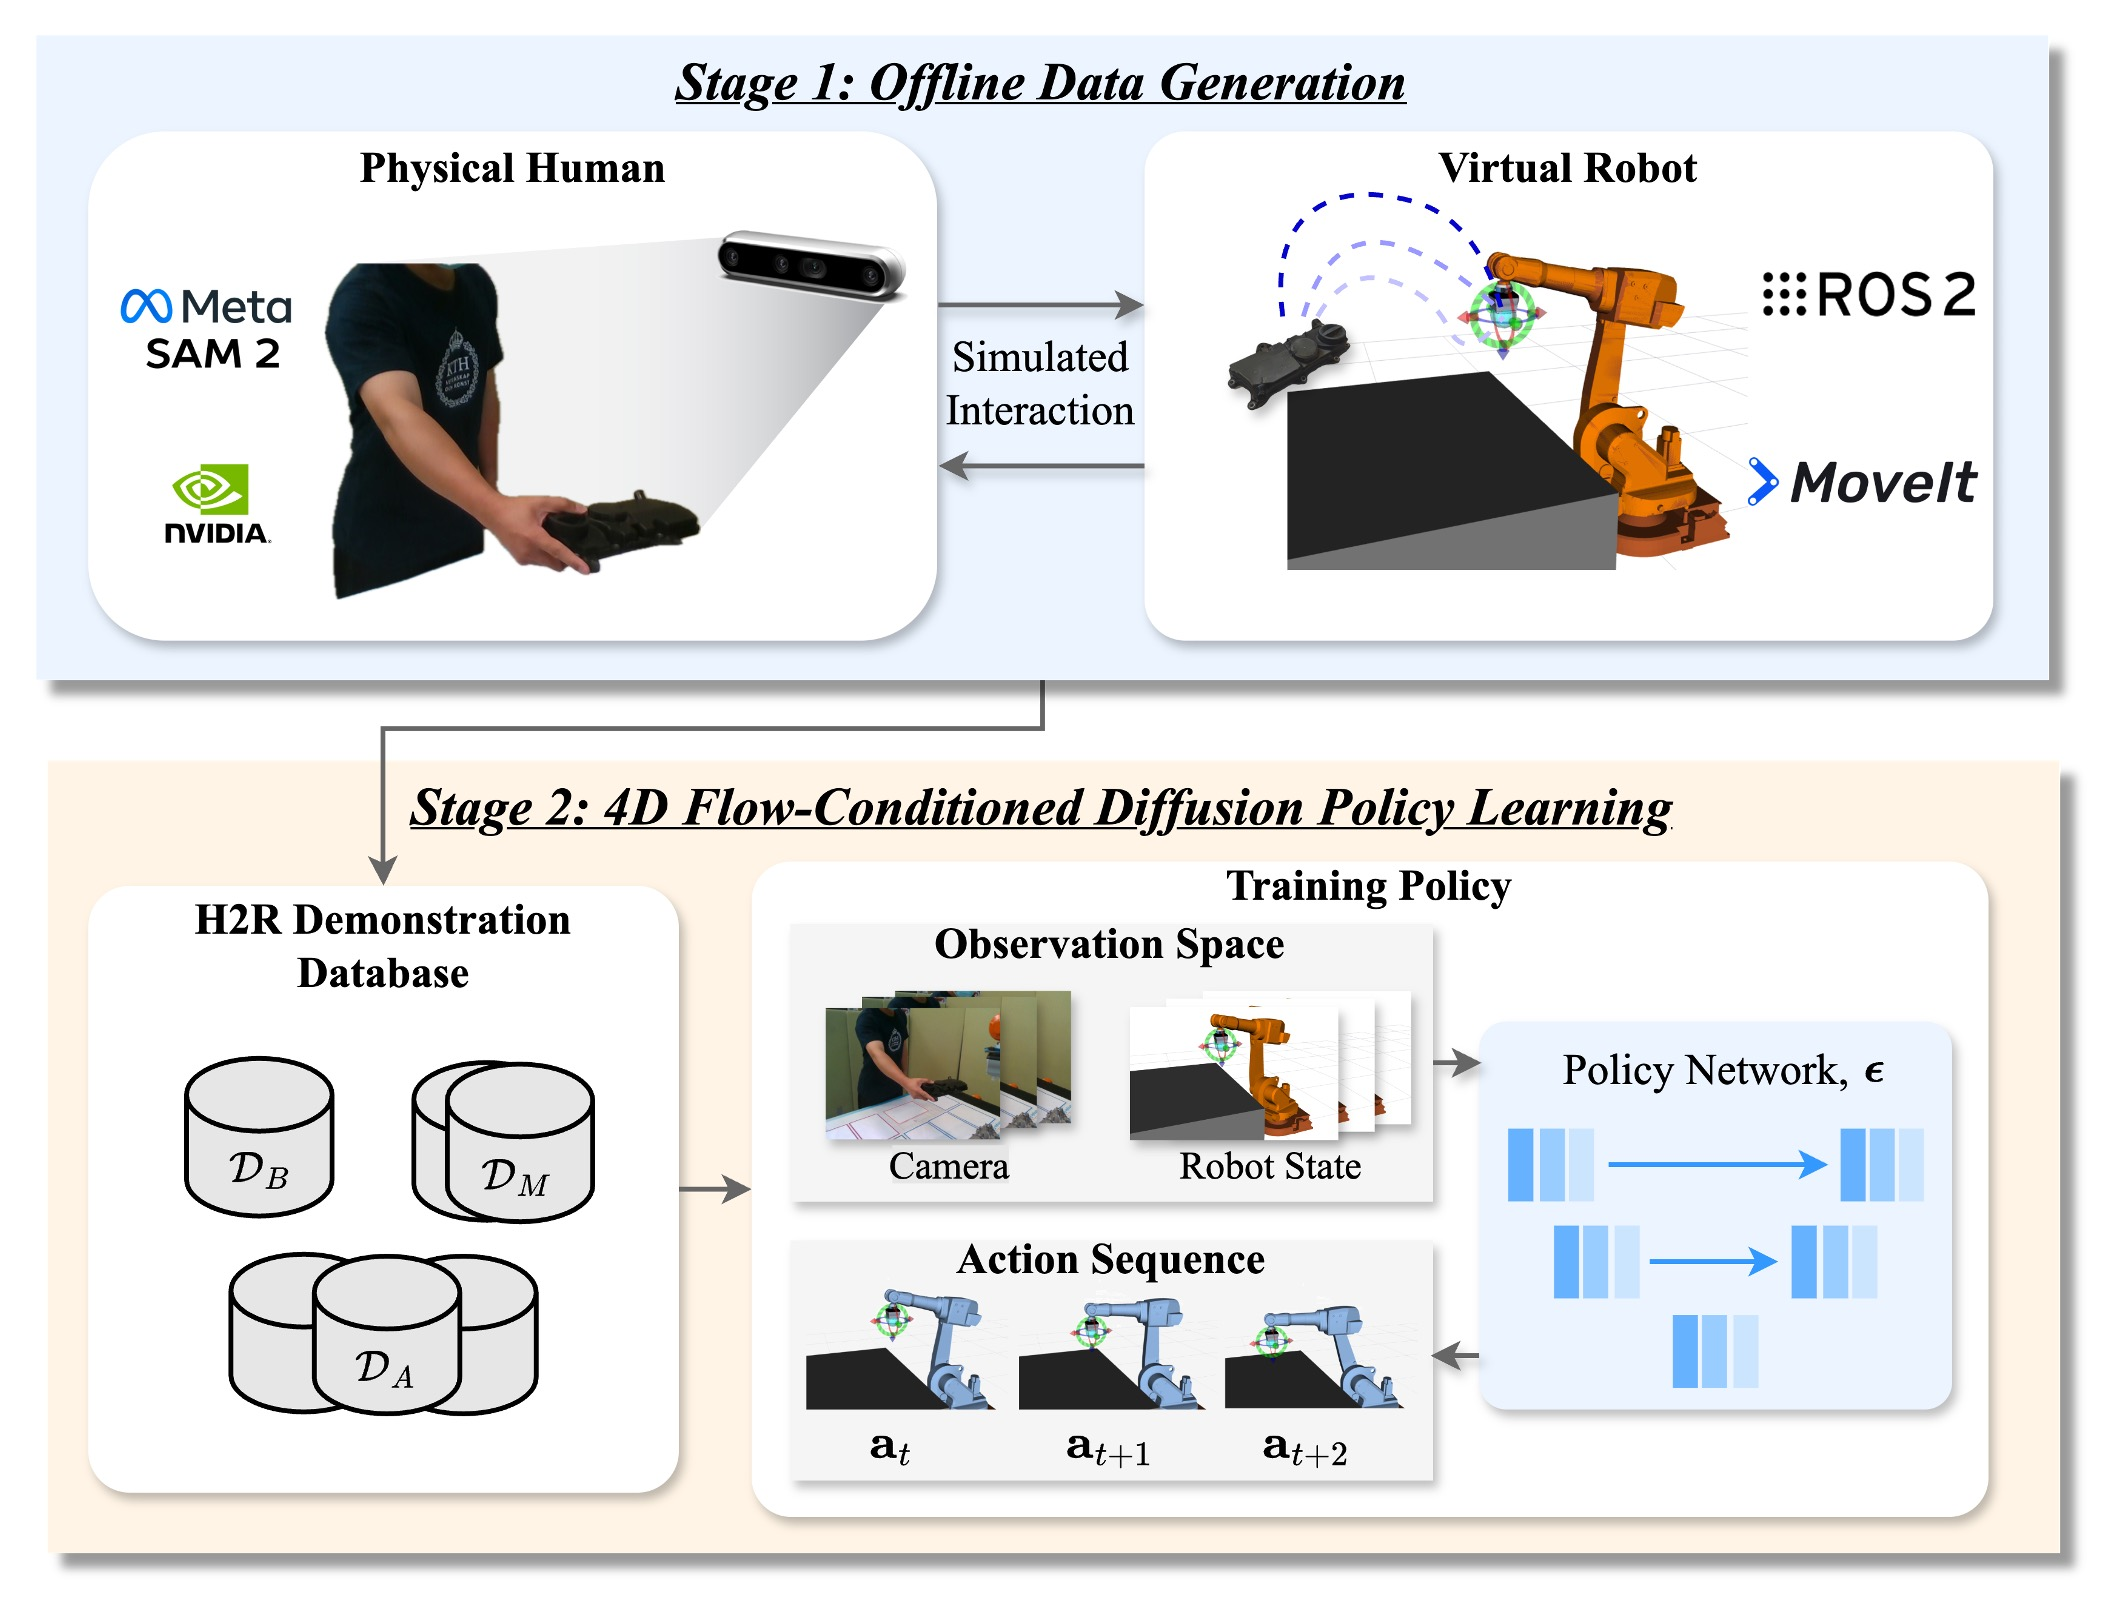
\includegraphics[width=\linewidth]{overall.jpg}
    \caption{Two-stage pipeline of the proposed framework for H2R object handover tasks.}
    \label{overall}
\end{figure}

The first stage of the proposed framework focuses on generating a large-scale and diverse dataset of H2R handover demonstrations without requiring a physical robot. This offline process begins with RGB-D video recordings of human-object handover scenarios. For each demonstration, we extract the final pose of the object using pretrained VFMs. Based on this final pose, we procedurally synthesize a variety of kinematically feasible and geometrically diverse robot trajectories using motion planning algorithms. By temporally aligning the captured human motion with these synthesized robot motions under a set of rule-based constraints, we construct a comprehensive dataset of paired H2R handover demonstrations. These demonstrations form the foundation for learning the handover policy in the second stage.

In the second stage, we formulate policy learning as a conditional generation problem, aiming to map structured observations of the human-object-robot interaction to future robot actions. To this end, we construct a novel 4D spatiotemporal flow representation that integrates a skeletal kinematic flow and a geometric motion flow, jointly providing a compact and expressive conditioning context for the policy. Based on this representation, our STFlowH2R is trained to generate reliable and context-aware robot actions. By decoupling data acquisition from real-world execution and leveraging rich spatiotemporal cues, this framework enables efficient, scalable, and robust policy learning for H2R object handover tasks.

\begin{table}[htbp]
\centering
\scriptsize
\caption{Important symbols.}
\label{symbols}
\begin{tabular}{ll}
\toprule
\textbf{Symbol} & \textbf{Description} \\
\midrule
$N_H$                           & Number of human demonstrations \\
$N_R$                           & Number of synthesized robot trajectories per human demo\\
$N_S$                           & Number of temporal augmentations per trajectory \\
$T_o$                           & Observation horizon \\
$T_p$                           & Prediction horizon \\
$T_a$                           & Action execution horizon \\
$T_i^{j}$                       & Length of $j$-th robot trajectory for $i$-th demo \\
$\mathbf{v}_i^T$                & Target point position of object in $i$-th demo \\
$\boldsymbol{\tau}_i^j$         & $j$-th robot trajectory for $i$-th human demo \\
$\mathcal{O}_{i}^{p}$           & Temporally shifted observation sequence \\
$\mathcal{D}_B$                 & Basic dataset \\
$\mathcal{D}_M$                 & Multi-trajectory dataset \\
$\mathcal{D}_A$                 & Augmented dataset \\
$\mathbf{J}^H$, $\mathbf{J}^R$  & Human and robot 3D joint coordinates \\
$\mathbf{D}_H$, $\mathbf{D}_R$  & Adjacency matrices of human and robot kinematic graphs \\
$\mathcal{P}$                   & Raw point cloud flow \\
$\hat{\mathcal{P}}$             & Geometric motion flow \\
$\mathcal{F}_S$                 & Skeletal kinematic flow encoder \\
$\mathcal{F}_G$                 & Geometric motion flow encoder \\
$\bm{f}_S$                      & Kinematic flow embedding \\
$\bm{f}_G$                      & Geometric flow embedding \\
$\bm{f}$                        & Fused flow embedding \\
$\mathbf{A}$                    & Predicted robot action \\
$d_C$                           & Feature dimension output from the TCN \\
$d_G$                           & Feature dimension output from the GAT \\
$d_P$                           & Feature dimension output from the geometric motion flow encoder \\
$d_A$                           & Action dimension \\
$K$                             & Number of diffusion steps \\
$\boldsymbol{\epsilon}_\theta$  & Noise prediction network of the diffusion policy \\
$\mathbf{A}_k$                  & Noisy action at diffusion step $k$ \\
$\mathbf{c}$                    & Conditioning vector \\
$\mathbf{e}_k$                  & Diffusion timestep embedding \\
$\boldsymbol{\gamma}, \boldsymbol{\beta}$ & FiLM modulation parameters \\
\bottomrule
\end{tabular}
\end{table}


\subsection{Offline Data Generation via Simulated Human-robot Interaction}  \label{sec:3.2}
To enable policy learning without requiring costly physical interactions, we propose a simulated data generation pipeline that constructs large-scale, high-quality H2R handover demonstrations in a fully offline and physical robot-free manner, as shown in Fig.~\ref{data_pipeline}. This process consists of three key parts: (1) estimating the final object pose from human demonstrations using VFMs, (2) synthesizing kinematically valid and diverse robot trajectories by sampling initial poses and perturbing intermediate control points, and (3) temporally aligning human and robot motions through rule-based augmentation. The resulting dataset provides rich and realistic training samples for downstream policy learning.


\begin{figure*}[!htb]
    \centering
    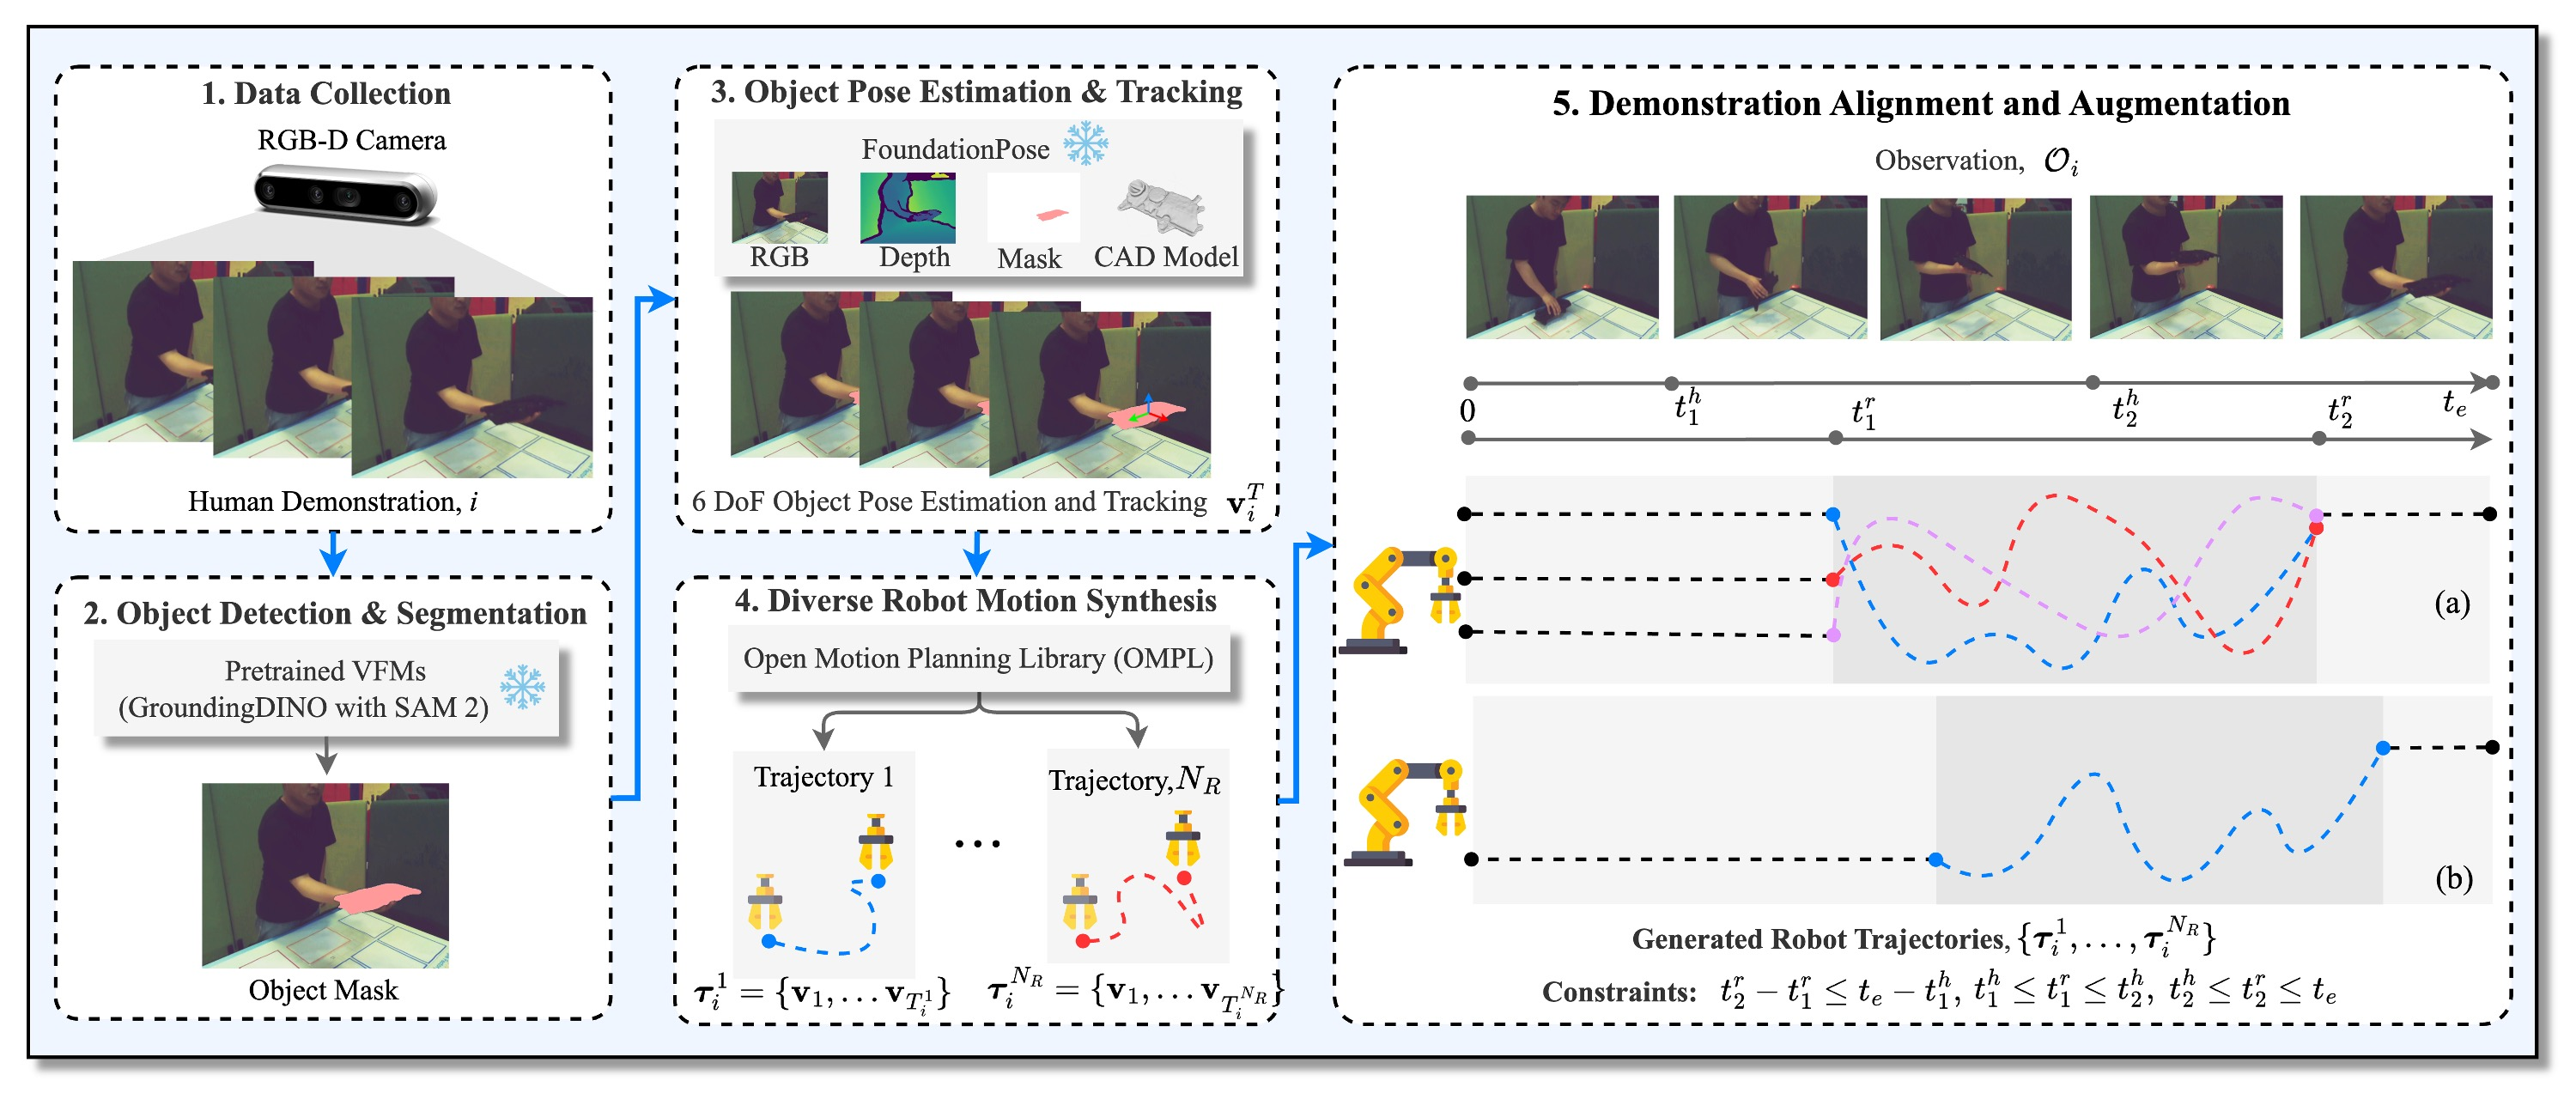
\includegraphics[width=\linewidth]{data_pipeline.jpg}
    \caption{An overview of our proposed offline physical robot-free data generation pipeline for IL in H2R object handover tasks. The process starts with (1) VFMs-based object pose estimation from human demonstration videos, followed by (2) diverse robot motion synthesis using OMPL, and concludes with (3) rule-based alignment and augmentation to create the final training dataset.}
    \label{data_pipeline}
\end{figure*}

\subsubsection{Pretrained VFMs-based object pose estimation}    \label{sec:3.2.1}
The foundation of robot trajectory synthesis lies in estimating the final pose of the handover object manipulated by the human. To this end, we utilize monocular RGB-D recordings of human-object interaction and employ VFMs to localize the target object in a zero-shot manner, thereby eliminating the need for object-specific detectors or manual annotations. Modern VFMs such as Grounding DINO~\cite{liu2024grounding} and SAM 2~\cite{ravi2024sam2} have demonstrated remarkable generalization in object grounding and segmentation tasks from natural language prompts. Thus, the object pose estimation pipeline comprises the following stages:
\begin{itemize}
    \item \textbf{Prompt-based object segmentation}: Given a user-defined textual description, such as “cover,” the VFMs segment the object of interest in the RGB frame and generate a precise 2D segmentation mask. This step yields a clean and focused region of interest for subsequent pose estimation.
    \item \textbf{Object pose estimation}: Using the segmented object mask, the corresponding RGB and depth images, and the 3D CAD model of the object, FoundationPose~\cite{wen2024foundationpose} is employed to estimate the object’s 6D pose with respect to the camera frame. To facilitate downstream robot motion planning, the estimated pose is transformed from the camera frame to the world coordinate frame using known extrinsic calibration parameters.
\end{itemize}

Consequently, both the object pose and robot actions are represented as 3D translation vectors throughout the pipeline. More formally, the robot's action is defined as the target end-effector position vector $\mathbf{a}_t \in \mathbb{R}^3$. This 3-DoF action representation is sufficient for the industrial handover tasks under study. Specifically, let the dataset contain $N_H$ human demonstrations. For each demonstration $i \in \{ 1, 2, \dots, N_H \} $, the extracted handover readiness point defines a target point $\mathbf{v}_i^T$, which serves as the goal position for downstream robot trajectory synthesis.



\subsubsection{Diverse robot motion synthesis} \label{sec:3.2.2}

With the handover object’s pose trajectory estimated for each human demonstration, we synthesize a diverse set of kinematically valid robot motion trajectories to support robust policy learning. To construct a rich dataset of robot motions, we adopt a fully programmatic synthesis approach based on the Open Motion Planning Library (OMPL)~\cite{sucan2012open} and inverse kinematics, thereby avoiding the need for physical robots during data collection. For each human demonstration $i$, the target point $\mathbf{v}_i^T$ serves as the endpoint for all generated robot trajectories. The synthesis pipeline proceeds as follows:
\begin{itemize}
\item \textbf{Initial pose sampling:} For each trajectory, we randomly sample a valid initial end-effector position within a constrained workspace region, while keeping its orientation fixed. This sampling provides a range of distinct starting points for the corresponding target point $\mathbf{v}_i^T$ for human demonstration $i$.

\item \textbf{Control-point-based trajectory generation:} Given the sampled initial pose and the fixed target pose $\mathbf{v}_i^T$, a smooth 3D trajectory is generated using an intermediate control point. This control point is initially placed at the midpoint between the start and target positions. It is then perturbed laterally and vertically to introduce geometric diversity and ensure variability across trajectories.

\item \textbf{Trajectory execution and filtering:} The generated waypoints are passed to a motion planning interface, which internally performs inverse kinematics and trajectory planning via MoveIt 2. If the robot successfully reaches all waypoints, the trajectory is accepted and stored; otherwise, the attempt is discarded. This implicit filtering ensures that only physically valid and executable trajectories are retained in the dataset.

\end{itemize}

By repeating this process across multiple initializations and control-point perturbations, we synthesize a diverse and physically executable set of robot trajectories for each human demonstration. Specifically, for each demonstration $i$, we generate $N_R$ robot trajectories, resulting in a set of sequences $\{ \boldsymbol{\tau}_{i}^{j} \}_{j=1}^{N_R}$. Each trajectory is defined as:

\begin{equation}
    \boldsymbol{\tau}_{i}^{j} = \{ \mathbf{v}_1, \mathbf{v}_2, \dots, \mathbf{v}_{T_{i}^{j}} \},
\end{equation}
where $T_{i}^{j}$ denotes the number of waypoints in the $j$-th trajectory associated with the $i$-th human demonstration. All trajectories in $\{ \boldsymbol{\tau}_{i}^{j} \}$ terminate at the same target position $\mathbf{v}_i^T$, while differing in path geometry and duration. This diversity is crucial for enabling the learned policy to generalize across varying motion paths, initial poses, and human handover behaviors.

At this stage, we define two intermediate datasets based on the synthesized robot trajectories. The basic dataset $\mathcal{D}_B$ consists of $N_H$ human demonstrations, each paired with a single synthesized robot trajectory, namely the first in the set, forming a minimal one-to-one correspondence without spatial or temporal variation. The multi-trajectory dataset $\mathcal{D}_M$ extends this by including all $N_R$ synthesized trajectories per human demonstration, resulting in a dataset of size $N_H \times N_R$ that captures diverse spatial realizations for the same human input.

\subsubsection{Rule-based demonstrations alignment and augmentation}    \label{sec:3.2.3}
Although a diverse set of robot trajectories has been generated for each human demonstration, simply concatenating these trajectories with the corresponding human motions is insufficient for constructing realistic handover demonstrations. This is because the relative timing between the human's handover presentation and the robot's response plays a critical role in ensuring natural and effective interaction. To address this, we introduce a rule-based temporal alignment and augmentation strategy that produces a large-scale dataset of temporally coherent and physically plausible H2R object handover demonstrations.

First, we manually annotate two key temporal events in each captured human motion sequence. The handover initiation point $t_1^H$, marks the moment the human begins moving the object with the clear intent to hand it over. The handover readiness point $t_2^H$, corresponds to the moment when the object's motion stabilizes, indicating that the human is ready for the robot to take the object. We also define $t_E$ as the termination point of the handover action, typically when the human begins retracting their hand.

Then, each synthesized robot trajectory is associated with its own start and end timestamps: robot motion initiation $t_{1}^R$ and robot motion termination $t_2^R$. To ensure temporal compatibility between the human and robot motions, the following alignment constraints are imposed:
\begin{gather}
    t_2^R -t_1^R \leq t_E - t_1^H,  \label{c1} \\
    t_1^H \leq t_1^R \leq t_2^H,  \label{c2} \\
    t_2^H \leq t_2^R \leq t_E. \label{c3}
\end{gather}

Constraint~\ref{c1} ensures that the robot’s motion duration does not exceed the available interaction window. Constraint~\ref{c2} ensures that the robot initiates its motion after the human has initiated the handover but before the human is ready, allowing the policy to learn both reactive and anticipatory behaviors. Constraint~\ref{c3} guarantees that the robot completes its action while the human is still holding the object in a stable, ready-for-transfer pose.

To augment the dataset, we generate multiple temporally aligned sequences from each synthesized pair of human and robot motions. Specifically, for each human demonstration $i$ and each corresponding robot trajectory $j$, we further introduce $N_S$ temporal variations by randomly sampling different robot start times. That is, for each pairing $(i, j)$, we generate $N_S$ temporally distinct alignments indexed by $p \in \{1, \dots, N_S\}$. The robot motion initiation time $t_1^{R}$ is sampled uniformly from the human handover interval, i.e., $t_1^R \sim U(t_1^H, t_2^H)$. Then, the corresponding termination time is computed as $t_2^R = t_1^R + T_{i}^{j}$. If both $t_1^R$ and $t_2^R$ satisfy the alignment constraints~\ref{c1} and \ref{c3}, the alignment is retained to form a new training sequence.

As a result, from a relatively small number of recorded human motions and synthesized robot trajectories, we construct a large-scale dataset that captures a wide range of spatial and temporal interaction patterns. The augmented dataset is denoted as:
\begin{equation}
\mathcal{D}_A = \left\{ \left( \mathcal{O}_{i}^{p}, \boldsymbol{\tau}_{i}^{j} \right) \,\middle|\, 1 \leq i \leq N_H,\ 1 \leq j \leq N_R,\ 1 \leq p \leq N_S \right\},
\end{equation}
where $\mathcal{O}_{i}^{p}$ denotes the temporally shifted observation sequence from the $i$-th human demonstration under the $p$-th alignment configuration, and $\boldsymbol{\tau}_{i}^{j}$ is the associated robot trajectory. This temporally enriched pairing strategy plays a critical role in training a policy that is robust to variations in interaction timing and dynamic coordination.


This procedure enables the generation of diverse, temporally varied, and physically consistent handover demonstrations. As a result, from a relatively small number of recorded human motions and synthesized robot trajectories, we construct a large-scale dataset that captures a wide range of spatial and temporal interaction patterns.



\subsection{Learning the 4D spatiotemporal flow-conditioned diffusion policy}  \label{sec:3.3}
To generate natural and context-aware robot behaviors for H2R object handovers, it is essential to model the underlying spatiotemporal structure of interaction and leverage it to guide the policy learning process. To achieve this, we introduce our STFlowH2R that leverages a conditional DM conditioned on a comprehensive 4D spatiotemporal flow representation, as illustrated in Fig.~\ref{diffusion}. This section details the three core components of our policy learning module: (1) the formulation of a skeletal kinematic flow to model the high-level kinematic evolution of the human-robot system; (2) the design of a geometric motion flow to capture fine-grained geometric dynamics; and (3) the architecture of the conditional DM that generates robot action sequences by mapping these powerful representations to the robot's action space. This design enables STFlowH2R to develop a deep understanding of the interactive dynamics, leading to anticipatory and context-aware behaviors.



\begin{figure*}[!htb]
    \centering
    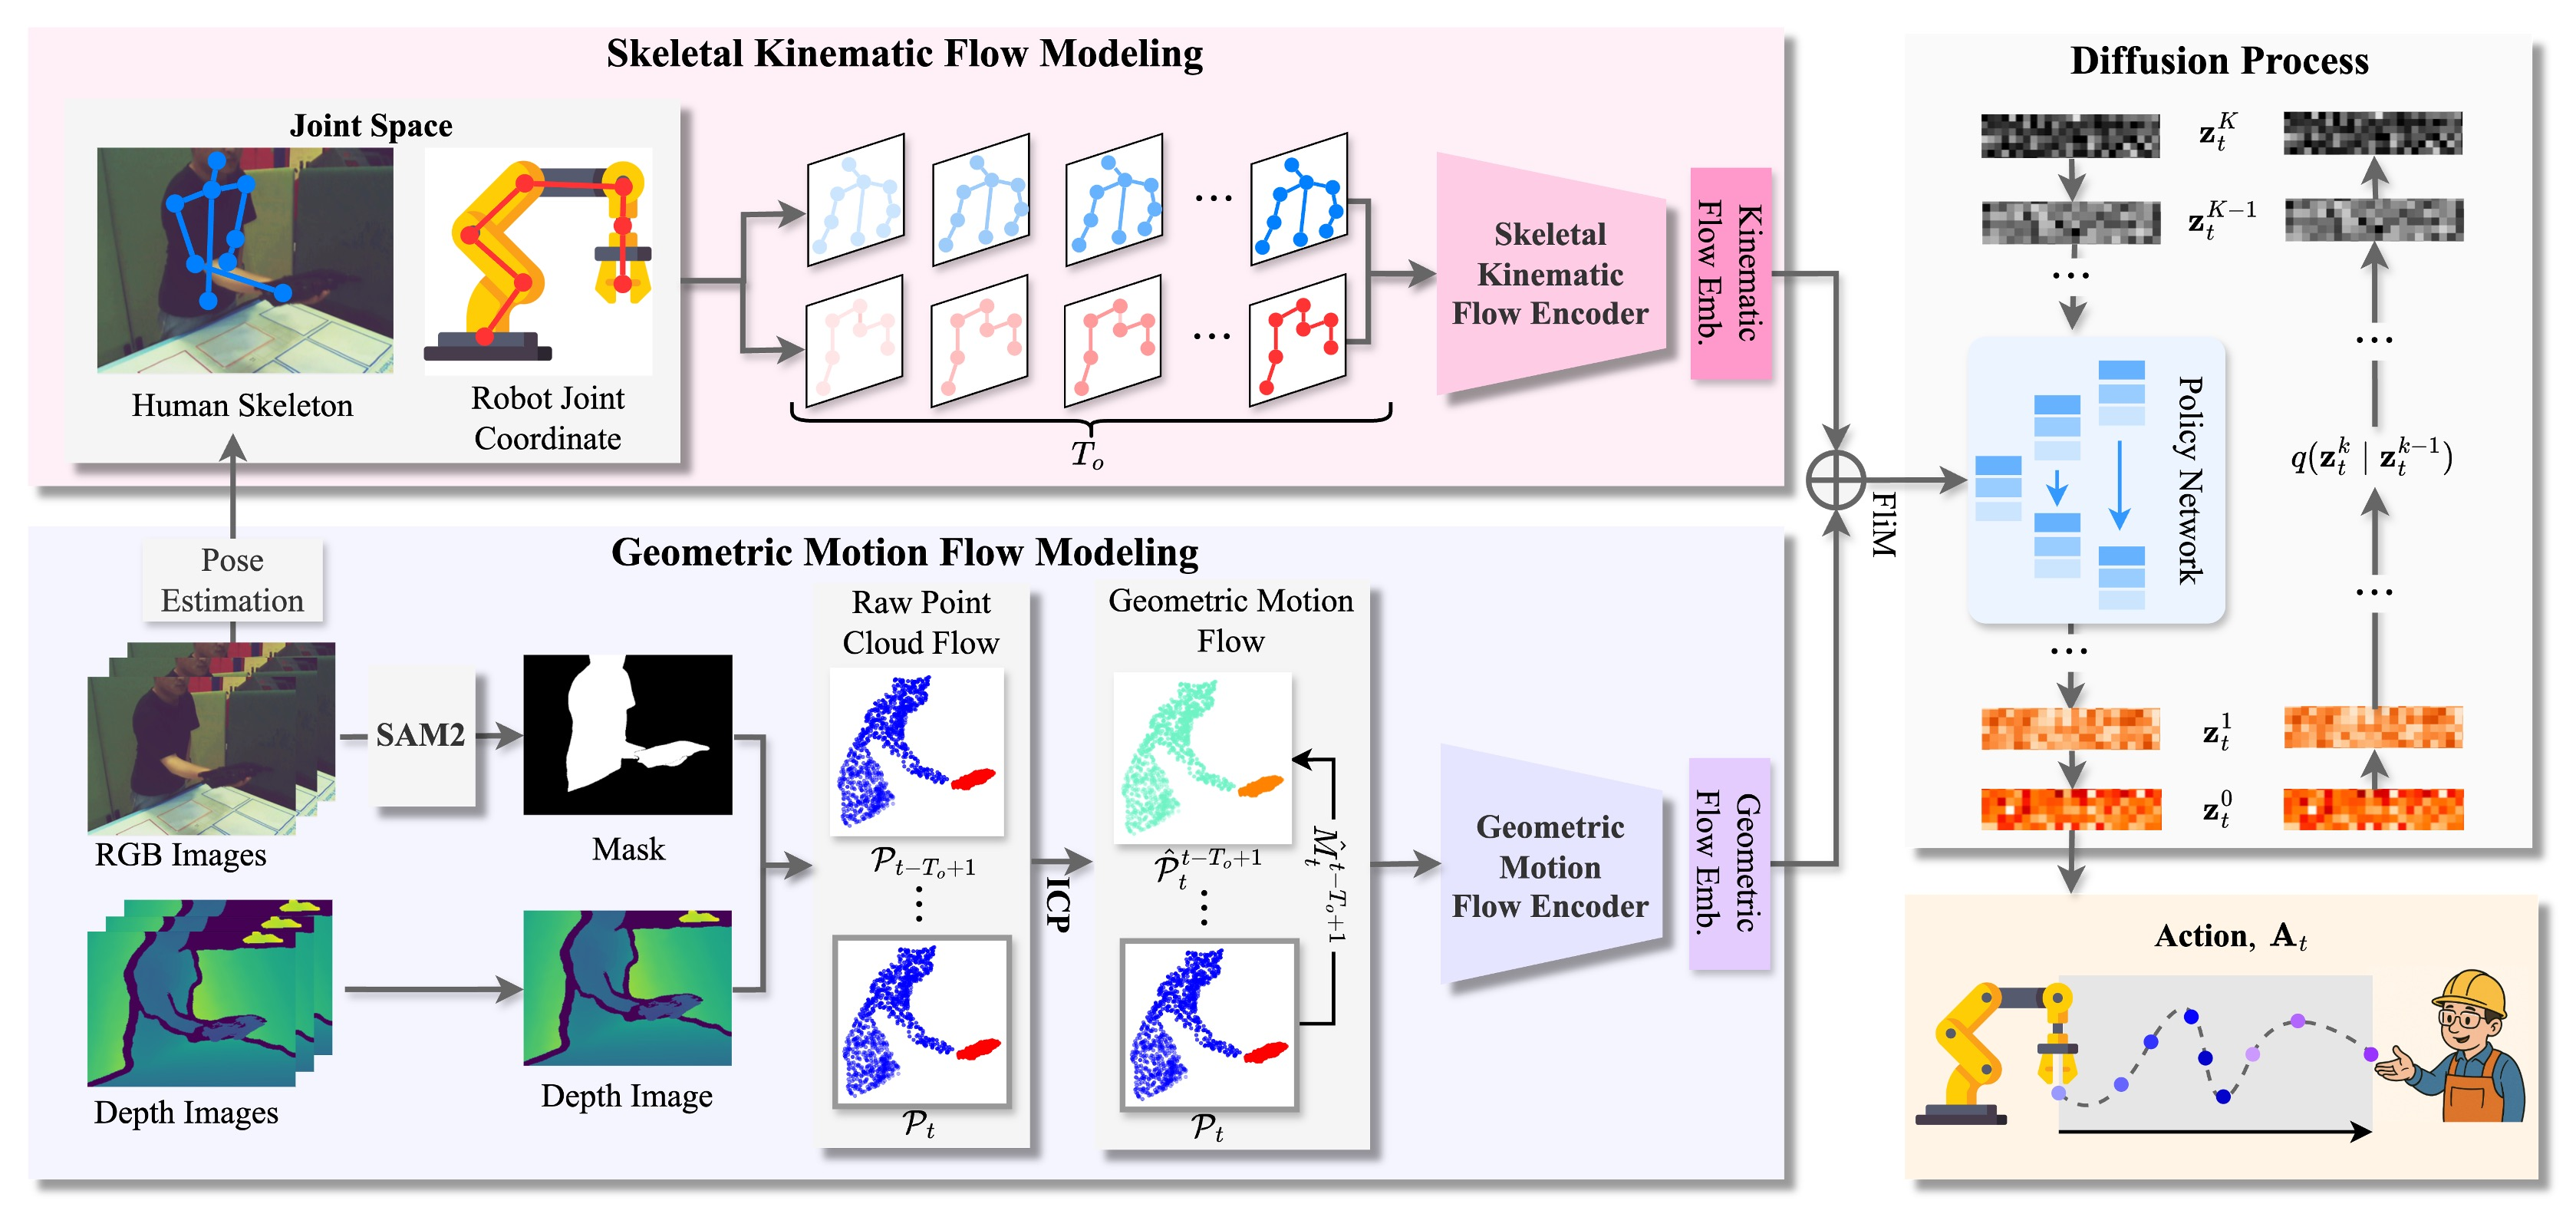
\includegraphics[width=\linewidth]{diffusion.jpg}
    \caption{The architecture of our proposed STFlowH2R policy for H2R object handover tasks. The model takes raw joint data from humans and robots, along with point clouds, as input. These are processed by the skeletal kinematic flow encoder and the geometric motion flow encoder, respectively. The resulting fused 4D spatiotemporal flow embedding is used to condition a U-Net-based DM, which generates the robot action sequence.}
    \label{diffusion}
\end{figure*}

\subsubsection{Skeletal kinematic flow modeling}    \label{sec:3.3.1}
A fundamental requirement for learning a robust and natural handover policy is the ability to jointly model the spatial relationships and temporal dynamics of human–robot interactions. To this end, we propose the skeletal kinematic flow encoder, denoted as $\mathcal{F}_S$, which encodes the raw motion trajectories of the human and the robot into a unified and expressive representation, as illustrated in Fig.~\ref{STEncoding}.

\begin{figure*}[htbp]
    \centering
    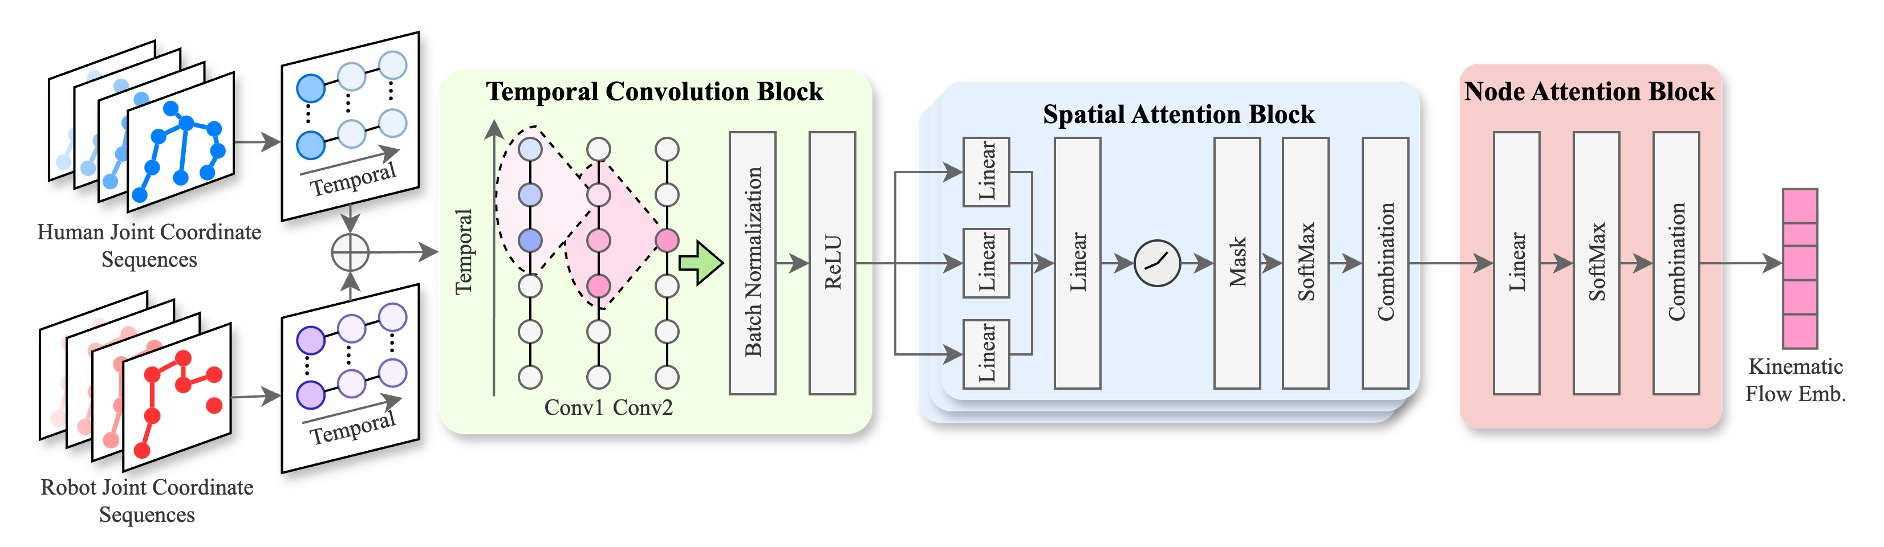
\includegraphics[width=\linewidth]{STEncoding.jpg}
    \caption{Detailed architecture of the skeletal kinematic flow encoder $\mathcal{F}_S$. The encoder first uses a TCN to capture local motion features for each joint. Subsequently, a GAT models the spatial dependencies within the unified human-robot spatial graph. The final features are aggregated using node-level attention pooling.}
    \label{STEncoding}
\end{figure*}

The encoder takes as input the 3D joint coordinates of the human and the robot, denoted as $\mathbf{J}^H \in \mathbb{R}^{T_o \times J_H \times 3}$ and $\mathbf{J}^R \in \mathbb{R}^{T_o \times J_R \times 3}$, respectively, over an observation horizon of length $T_o$, where $J_H$ and $J_R$ represent the number of joints for the human and the robot. The kinematic structures of both agents are defined by their respective adjacency matrices, $\mathbf{D}_H$ and $\mathbf{D}_R$. At each time step $t$, we construct a unified spatial graph by stacking the joint positions:
\begin{equation}
    \mathbf{J} = \begin{bmatrix}
\mathbf{J}^H_t \\
\mathbf{J}^R_t
\end{bmatrix}\in\mathbb{R}^{J_T \times 3}, A = \begin{pmatrix}
\mathbf{D}_H & 0 \\
0 & \mathbf{D}_R
\end{pmatrix}\in\mathbb{R}^{J_T \times J_T}
\end{equation}
where $J_T = J_H + J_R$ denotes the total number of joints. 

To process this unified representation, the skeletal kinematic flow encoder $\mathcal{F}_S$ employs two key modules, including a Temporal Convolutional Network (TCN) for capturing local motion dynamics across time, and a Graph Attention Network (GAT) for modeling spatial dependencies among joints at each time step. First, the TCN is applied to model the temporal evolution of each joint independently over time. Using stacked 1D causal convolutions, the network ensures that each output depends solely on current and past inputs, which is critical for enabling responsive behavior in physical human-robot interaction. By capturing short-term motion patterns within joint trajectories, the TCN enriches the representation with informative temporal context. 

Formally, let $\mathbf{x}_k \in \mathbb{R}^{T_o \times 3}$ denote the temporal trajectory of the $k$-th joint in $\mathbf{J}$, where $k \in \{ 1, 2, \dots, J_T \}$. For each joint, the TCN applies a stack of 1D causal convolutional layers along the temporal dimension to extract local motion features. The output of the $l$-th layer is computed as:
\begin{equation}
    \mathbf{x}_k^{(l)} = \sigma \left( \operatorname{Conv1D} \left( \mathbf{x}_k^{(l-1)} \right) \right),
\end{equation}
where $\mathbf{x}_k^{(0)} = \mathbf{x}_k$, $\text{Conv1D}(\cdot)$ denotes a 1D causal convolution, and $\sigma(\cdot)$ is the activation function. All joints share the same convolutional parameters, and appropriate padding ensures the temporal resolution is preserved. After $L$ layers, we obtain a temporally enriched sequence $\mathbf{X} = \{ \mathbf{x}_1^{(L)}, \mathbf{x}_2^{(L)}, \dots, \mathbf{x}_{J_T}^{(L)} \}$, where each $\mathbf{x}_k^{(L)} \in \mathbb{R}^{T_o \times d_C}$, where $d_C$ is the feature dimension produced by the TCN. For each time step $t$, the features of all joints are aggregated into a graph-level representation $\mathbf{g}_t \in \mathbb{R}^{J_T \times d_C}$, which is then passed to the spatial encoder for relational modeling via GAT.


Subsequently, the GAT is employed on the unified spatial graph at each time step to model relational features. To progressively capture higher-order spatial dependencies, we stack $M$ GAT layers. The feature vector of node $i$ at layer $m \in \{ 1, \dots, M \}$ is denoted by $\mathbf{u}_i^{(m)}$. The input to the first layer, $\mathbf{u}_i^{(0)} \in \mathbb{R}^{d_C}$, corresponds to the temporally-enriched feature from the TCN. For each layer $m$, the model updates node representations based on an attention mechanism. The attention coefficient $\mathbf{e}_{ij}^{(m)}$ between two connected nodes $i$ and $j$ at layer $m$ is computed using the features from the previous layer $m-1$:
\begin{equation}
    \mathbf{e}_{ij}^{(m)} = \operatorname{LeakyReLU} ((\boldsymbol{\alpha}^{(m)})^{\text{T}} \left[ \mathbf{W}^{(m)} \mathbf{u}_i^{(m-1)} \parallel \mathbf{W}^{(m)} \mathbf{u}_j^{(m-1)} \right])
\end{equation}
where $\mathbf{u}_i^{(m-1)}$ and $\mathbf{u}_j^{(m-1)}$ are the feature vectors from layer $m-1$, $\mathbf{W}^{(m)}$  is a learnable linear transformation, $\boldsymbol{\alpha}^{(m)}$ is a learnable weight vector that parameterizes the attention mechanism at layer $m$, and $\parallel$ denotes vector concatenation. The resulting attention scores are normalized via a softmax function to produce the final attention weights $\boldsymbol{\alpha}_{ij}^{(m)}$. The updated representation for node $i$ at layer $m$ is then computed as an aggregated sum of its neighbors’ transformed features, weighted by these attention scores:
\begin{equation}
    \mathbf{u}_i^{(m)} = \sigma\left( \sum_{j \in \mathcal{N}(i)} \alpha_{ij}^{(m)} \mathbf{W}^{(m)} \mathbf{u}_j^{(m-1)} \right),
\end{equation}
where $\mathcal{N}(i)$ denotes the set of neighbors of node $i$, and $\sigma(\cdot)$ is the activation function. This layer-wise propagation is repeated for $M$ layers, resulting in refined node features $\mathbf{u}_i^{(M)}$. To enhance stability and model expressiveness, multi-head attention is applied within each GAT layer.

The final output of the GAT layer at time step $t$ is the set of node features, $ \{ \mathbf{u}_1^{(M)}, \dots, \mathbf{u}_{J_T}^{(M)} \} \in \mathbb{R}^{J_T \times d_G}$, where $d_G$ denotes the feature dimension produced by the GAT. After passing through the temporal and spatial encoding layers, the features from all $J_T$ joints are aggregated at each time step using a node-level attention pooling mechanism. This layer computes attention weights over all joints and performs a weighted sum to produce a compact vector $\mathbf{u}_t^\prime \in \mathbb{R}^{d_G}$ that encapsulates the global spatial state of the human–robot system at time $t$.

Collecting these vectors across the observation horizon yields the kinematic flow embedding, defined as $\bm{f}_S = \{ \mathbf{u}_{t-T\_o + 1}^\prime, \dots, \mathbf{u}_{t}^\prime \} \in \mathbb{R}^{T_o \times d_G}$. This representation serves as a conditional context for the downstream STFlowH2R policy.



\subsubsection{Geometric motion flow modeling}  \label{sec:3.3.2}
While the skeletal kinematic flow effectively captures high-level kinematics, it abstracts away the fine-grained geometric details crucial for robust interaction. To address this limitation and capture the nuanced evolution of the object's pose and surface relative to the human, we introduce geometric motion flow modeling. Specifically, we first isolate the point clouds of the human and the handover object using a semantic segmentation model, focusing only on the relevant agents of interaction. Next, to explicitly represent motion and ensure temporal consistency, all past point clouds within the observation window are aligned to the coordinate system of the most recent frame using the Iterative Closest Point (ICP) algorithm~\cite{4767965}. Finally, this sequence of temporally-aligned point clouds is encoded by a geometric motion flow encoder $\mathcal{F}_G$ to generate a compact feature representation, the geometric motion flow $\bm{f}_G$.

First, for each frame within an observation horizon of length $T_o$, we process the RGB-D data to isolate the interacting agents. We utilize a segmentation model SAM2~\cite{ravi2024sam2} on the RGB image to generate two distinct, class-aware segmentation masks: one for the human and another for the object. The union of these two masks identifies the total region of interest. These masks are then applied to the corresponding depth map, allowing us to back-project only the relevant pixels into point clouds, $\mathbf{P}_t \in \mathbb{R}^{N_P \times 3}$. This procedure yields the raw point cloud flow, $ \mathcal{P} =  \{ \mathbf{P}_{t - T_o +1}, \mathbf{P}_{t - T_o +2}, \dots, \mathbf{P}_t \}$, representing the combined geometry of the human and object over the observation horizon.

Next, to explicitly model the motion of the interaction surfaces, we construct the geometric motion flow by aligning all historical point clouds to the coordinate system of the most recent frame. Let the point cloud at the current timestep $t$, $\mathbf{P}_t$, be the reference point cloud. The sequence of past point clouds, $\{ \mathbf{P}_{t-T_o+1}, \dots, \mathbf{P}_{t-1} \}$, constitutes the target point clouds. We then employ the ICP algorithm to register each target cloud $\mathbf{P}_i$, where $t- T_o + 1 \leq i < t$, to the reference point cloud $\mathbf{P}_t$. The optimal rigid transformation $\mathbf{M}_i^t$ is computed by ICP. This transformation consists of a rotation $\mathbf{R}_i^t$ and a translation $\mathbf{d}_i^t$, designed to minimize the distance between the transformed target cloud and its nearest neighbors in the reference cloud. This transformation is then applied to create the aligned point cloud:
\begin{equation}
\hat{\mathbf{P}}_i = \mathbf{M}_i^t (\mathbf{P}_i).
\end{equation}

Then, this process results in the geometric motion flow,  $ \hat{\mathcal{P}} = \{ \mathbf{\hat{P}}_{t-T_o+1}, \dots, \mathbf{\hat{P}}_{t-1}, \mathbf{\hat{P}}_{t} \}$ where all historical geometric data are represented in the current frame's perspective. Each aligned point cloud in this flow is then encoded into a compact feature vector using the geometric motion flow encoder $\mathcal{F}_G$, which is inspired by DP3~\cite{Ze2024DP3}. Specifically, per-point features are extracted using a series of fully connected layers with ReLU activations and Layer Normalization, and then globally aggregated via max pooling to obtain a permutation-invariant representation. This representation is passed through a final projection head to produce the embedding:
\begin{equation}
\mathbf{h}_i=\operatorname{Proj}\left(\max_{\mathbf{p}\in\mathbf{\hat{P}}_i}\left(\operatorname{MLP}(\mathbf{p})\right)\right),
\end{equation}
where $\mathbf{h}_i \in \mathbb{R}^{d_P}$ is the encoded representation of the aligned point cloud $\hat{\mathbf{P}}_i$, and $\operatorname{Proj} (\cdot)$ denotes a linear projection layer, mapping the aggregated feature to a fixed embedding dimension $d_P$.

The sequence of these feature vectors, $\bm{f}_G = \{ \mathbf{h}_{t-T_o+1}, \dots, \mathbf{h}_t \} \in \mathbb{R}^{T_o \times d_P}$, constitutes the geometric flow embedding. This rich, compact vector, capturing fine-grained geometric motion, serves as a crucial conditioning signal for our STFlowH2R policy, complementing the skeletal joint flow.


\subsubsection{Action generation with conditional diffusion model}  \label{sec:3.3.3}
With the kinematic flow embedding and the geometric motion embedding established, the final step of our methodology is to learn a policy that maps these rich representations to a sequence of robot actions. We formulate this policy using our STFlowH2R, a conditional DM exceptionally well-suited for generating smooth action trajectories. Our goal is to learn the conditional probability distribution $p \left( \mathbf{A} \mid \mathbf{c} \right)$, where $\mathbf{A} \in \mathbb{R}^{T_p \times d_A}$ is the robot's action over a prediction horizon $T_p$, and $\mathbf{c}$ is the conditioning context derived from our flow-based encoders over the observation horizon $T_o$.

The STFlowH2R policy is trained through both forward and reverse processes. In the forward process, we take a ground-truth robot action sequence $\mathbf{A}_0$ from our synthesized dataset and progressively corrupt it by adding Gaussian noise over $K$ discrete timesteps. The noisy action sequence $\mathbf{A}_k$ at any timestep $k \in \{1, \dots, K\}$ is sampled according to a fixed variance schedule $\beta_k$:
\begin{equation}
    \mathbf{A}_k = \sqrt{\overline{\alpha}_k} \mathbf{A}_0 + \sqrt{1 - \overline{\alpha}_k} \boldsymbol{\epsilon},
\end{equation}
where $\boldsymbol{\epsilon} \sim \mathcal{N}(0, \mathbf{I})$ is a noise vector, $\alpha_k = 1 - \beta_k$, and $\overline{\alpha}_k = \prod_{i=1}^k \alpha_i$. 
As $k$ approaches $K$, the distribution of $\mathbf{A}_k$ converges to a standard isotropic Gaussian distribution.


The conditioning context originates from the two feature sequences extracted from the observation horizon $T_o$: the kinematic flow embedding  $ \bm{f}_S \in \mathbb{R}^{T_o \times d_G} $ and the geometric flow embedding $ \bm{f}_G \in \mathbb{R}^{T_o \times d_P}$. These sequences are first concatenated along the feature dimension to create the fused flow embedding, $\bm{f}$: 
\begin{equation}
    \bm{f} = [ \bm{f}_S \parallel \bm{f}_G] \in \mathbb{R}^{T_o \times (d_G + d_P)}
\end{equation}

This fused sequence captures both the structured kinematics and fine-grained geometry of the interaction. To serve as a global condition, the features across the temporal dimension of this fused flow embedding $\bm{f}$ are concatenated to form the conditioning vector $ \mathbf{c}$. This operation preserves temporal order and feature richness, providing the noise prediction network with a comprehensive view of the observation horizon.

The conditional DM is instantiated as a U-Net-based noise prediction network $\boldsymbol{\epsilon}_\theta$. This architecture is particularly well-suited for generating coherent action trajectories due to its hierarchical structure, which captures temporal patterns at multiple scales, and its use of skip connections, which preserve fine-grained details throughout the denoising process. This design has been proven effective for modeling complex temporal dependencies in diffusion-based generative tasks~\cite{chi2023diffusion}. The network takes as input the noisy action $\mathbf{A}_k \in \mathbb{R}^{T_p \times d_A}$, where $k$ denotes the current diffusion timestep and $T_p$ is the prediction horizon. The conditioning vector $ \mathbf{c} $ is not concatenated to the input but is instead injected into the network through the Feature-wise Linear Modulation (FiLM) module~\cite{perez2018film}. At each block of the U-Net, the conditioning process is as follows. First, the discrete diffusion timestep $k$ is converted into the diffusion timestep embedding, $\mathbf{e}_k \in \mathbb{R}^{d_E}$, using sinusoidal positional embeddings. Next, the conditioning vector $ \mathbf{c} $ is concatenated with the diffusion timestep embedding, producing a unified time-aware conditioning feature. It is this time-aware conditioning feature that is passed through a lightweight MLP to generate the scale $ \boldsymbol{\gamma} $ and bias $\boldsymbol{\beta}$ parameters. These parameters then dynamically modulate the intermediate feature map $\mathbf{x}$:
\begin{equation}
    \text{FiLM}(\mathbf{x}) = \boldsymbol{\gamma} \odot \mathbf{x} + \boldsymbol{\beta},
\end{equation}
where $ \mathbf{x} $ is the intermediate feature map and $ \odot $ denotes element-wise multiplication. This modulation mechanism allows the time-aware conditioning feature to influence the denoising process hierarchically throughout the network.

The noise prediction network $\boldsymbol{\epsilon}_\theta$ is trained to predict the injected Gaussian noise. Concretely, we minimize the Mean Squared Error (MSE) between predicted noise and true noise:
\begin{equation}
    \mathcal{L}(\theta) = 
    \mathbb{E}_{\mathbf{A}_0, \mathbf{c}, \boldsymbol{\epsilon}, k}
    \left[
      \left\| 
        \boldsymbol{\epsilon} - \boldsymbol{\epsilon}_\theta(\mathbf{A}_k, k, \mathbf{c})
      \right\|^2
    \right],
\end{equation}
where $k$ is sampled uniformly from $\{1, \dots, K\}$, and $\mathbf{A}_k$ is constructed from $\mathbf{A}_0$ and $\boldsymbol{\epsilon}$ via the forward process.


At inference time, STFlowH2R generates an action by iteratively denoising an initial sample drawn from a standard Gaussian distribution $\mathbf{A}_K \sim \mathcal{N} (0, \mathbf{I})$ over $K$ steps to produce a clean action plan $\hat{\mathbf{A}}_0$ of length $T_p$. For real-time robot control, we employ a receding horizon control strategy. Specifically, we define a shorter action execution horizon $T_a < T_p$. In each control cycle, STFlowH2R observes the last $T_o$ steps of the interaction to generate a future action plan for $T_p$ steps. However, only the first $T_a$ actions from this plan are executed by the robot. After $T_a$ steps, a new observation is taken, and the process repeats. This encourages temporal action consistency across plans while allowing the robot to remain responsive to dynamic changes in the environment.


%% ------------------------------------------------------------------------------------------
\section{Experiments} \label{sec:4}
This section presents a comprehensive empirical evaluation of our proposed framework. We first detail the experimental setup in Section~\ref{exp_setup}, describe the dataset and baselines in Section~\ref{dataset}, and define the evaluation metrics in Section~\ref{metrics}. Finally, we present and analyze the results in Section~\ref{results}.


\subsection{Experimental setup} \label{exp_setup}

All experiments are conducted on a 6-DoF ABB IRB 1600 industrial robot arm equipped with an OnRobot VGC10 electric vacuum gripper, as shown in Fig.~\ref{exp_setting}. For perception, an Intel RealSense D435i camera is mounted on a table adjacent to the robot's workspace, providing a fixed eye-to-hand view of the interaction area. The camera captures RGB-D streams at 30 Hz with a resolution of 640 × 480. The robot control and perception pipelines are implemented using ROS 2, with MoveIt 2 providing the motion planning interface. All models are trained and executed on a workstation equipped with an NVIDIA RTX 4090 GPU.

\begin{figure}[htbp]
    \centering
    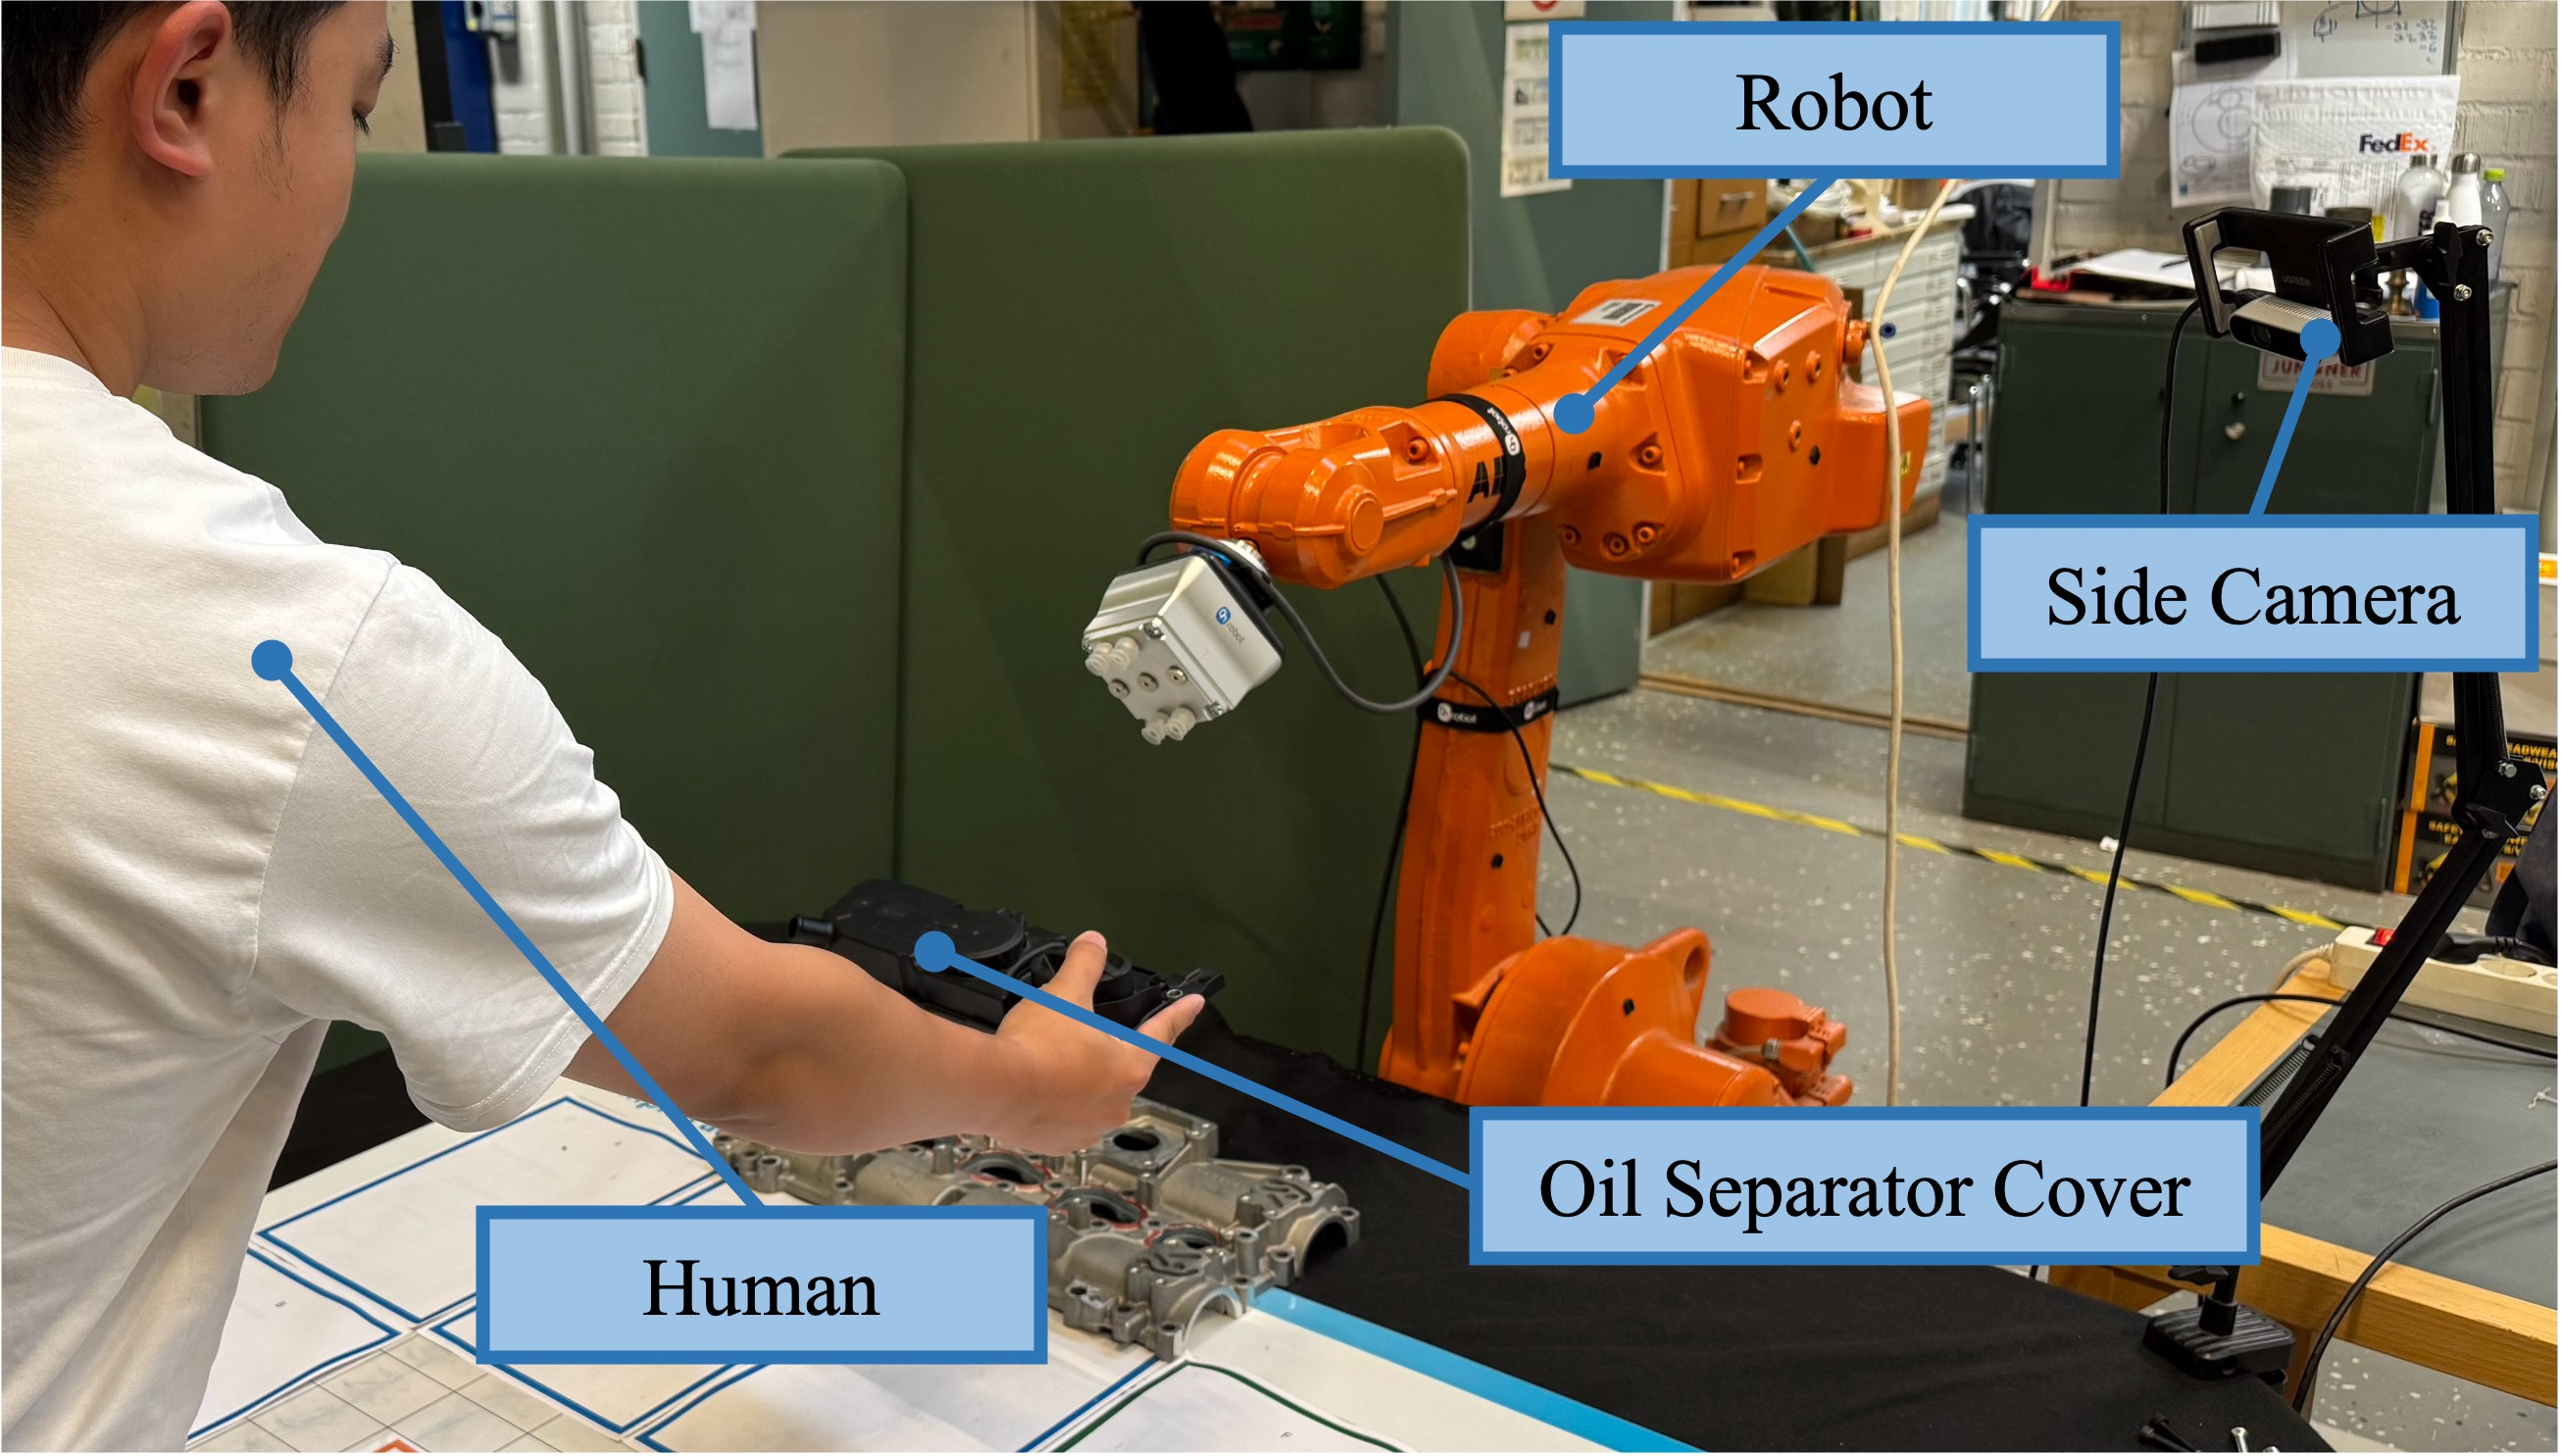
\includegraphics[width=0.8\linewidth]{exp_setting.jpg}
    \caption{ The physical experimental setup, featuring a 6-DoF ABB IRB 1600 industrial robot arm and a table-mounted Intel RealSense D435i camera in a fixed eye-to-hand configuration.}
    \label{exp_setting}
\end{figure}

Our proposed policy model, STFlowH2R, is implemented in PyTorch. Following DP3~\cite{Ze2024DP3}, we set the observation horizon to $T_o=2$, the prediction horizon to $T_p=4$, and the action execution horizon of $T_a=3$ for receding horizon control. The skeletal kinematic flow encoder utilizes a TCN with a kernel size of 3 to produce 256-dimensional temporal features. These are then processed by a 2-layer GAT with output dimensions of [256, 256] and [1, 4] attention heads per layer, respectively. The final output $d_G$ is a 256-dimensional feature vector. The geometric motion flow encoder processes down-sampled point clouds of 1024 points. It consists of a 3-layer MLP with hidden dimensions of [64, 128, 256] and LayerNorm. The final output $d_P$ is a 256-dimensional feature vector. The features from both encoders are concatenated to condition the DM. For training, we use a DDIM noise scheduler with 100 timesteps. This value is chosen to balance the trade-off between generation quality and inference speed; it provides high-quality action sequences while maintaining a latency suitable for real-time control, consistent with prior work in diffusion-based policies~\cite{chi2023diffusion}. The U-Net has downsampling dimensions of [128, 256, 384]. The model is trained for 3000 epochs using the AdamW optimizer with a learning rate of $1 \times 10^{-4}$ and a batch size of 128. We run each experiment with 3 different random seeds. The performance metrics reported in the results section are the mean and standard deviation across these three independent runs.


\subsection{Dataset description and baselines}  \label{dataset}

The dataset was constructed based on a specific industrial H2R handover task involving an oil separator cover. We collected a total of $N_H=80$ raw human demonstrations from 2 different participants. To evaluate the model's performance, these demonstrations were partitioned into a training set of 56 demonstrations and a test set of 24 demonstrations. The full augmented training dataset, $\mathcal{D}_A$, was generated by applying our offline data generation pipeline to the 56 training demonstrations. For each demonstration, we synthesized $N_R = 5$ diverse robot trajectories and applied $N_S = 5$ temporal alignments, resulting in a total of 1400 training samples. For ablation studies, we define two subsets, the basic dataset $\mathcal{D}_B$ with 56 samples and the multi-trajectory dataset $\mathcal{D}_M$ with 280 samples. The test set consists of the 24 raw, un-augmented demonstrations. As illustrated in Fig.~\ref{pose_dis}, the test set includes entirely novel handover configurations that were not observed during training, ensuring a rigorous evaluation of the policy's ability to generalize.


\begin{figure}
    \centering
    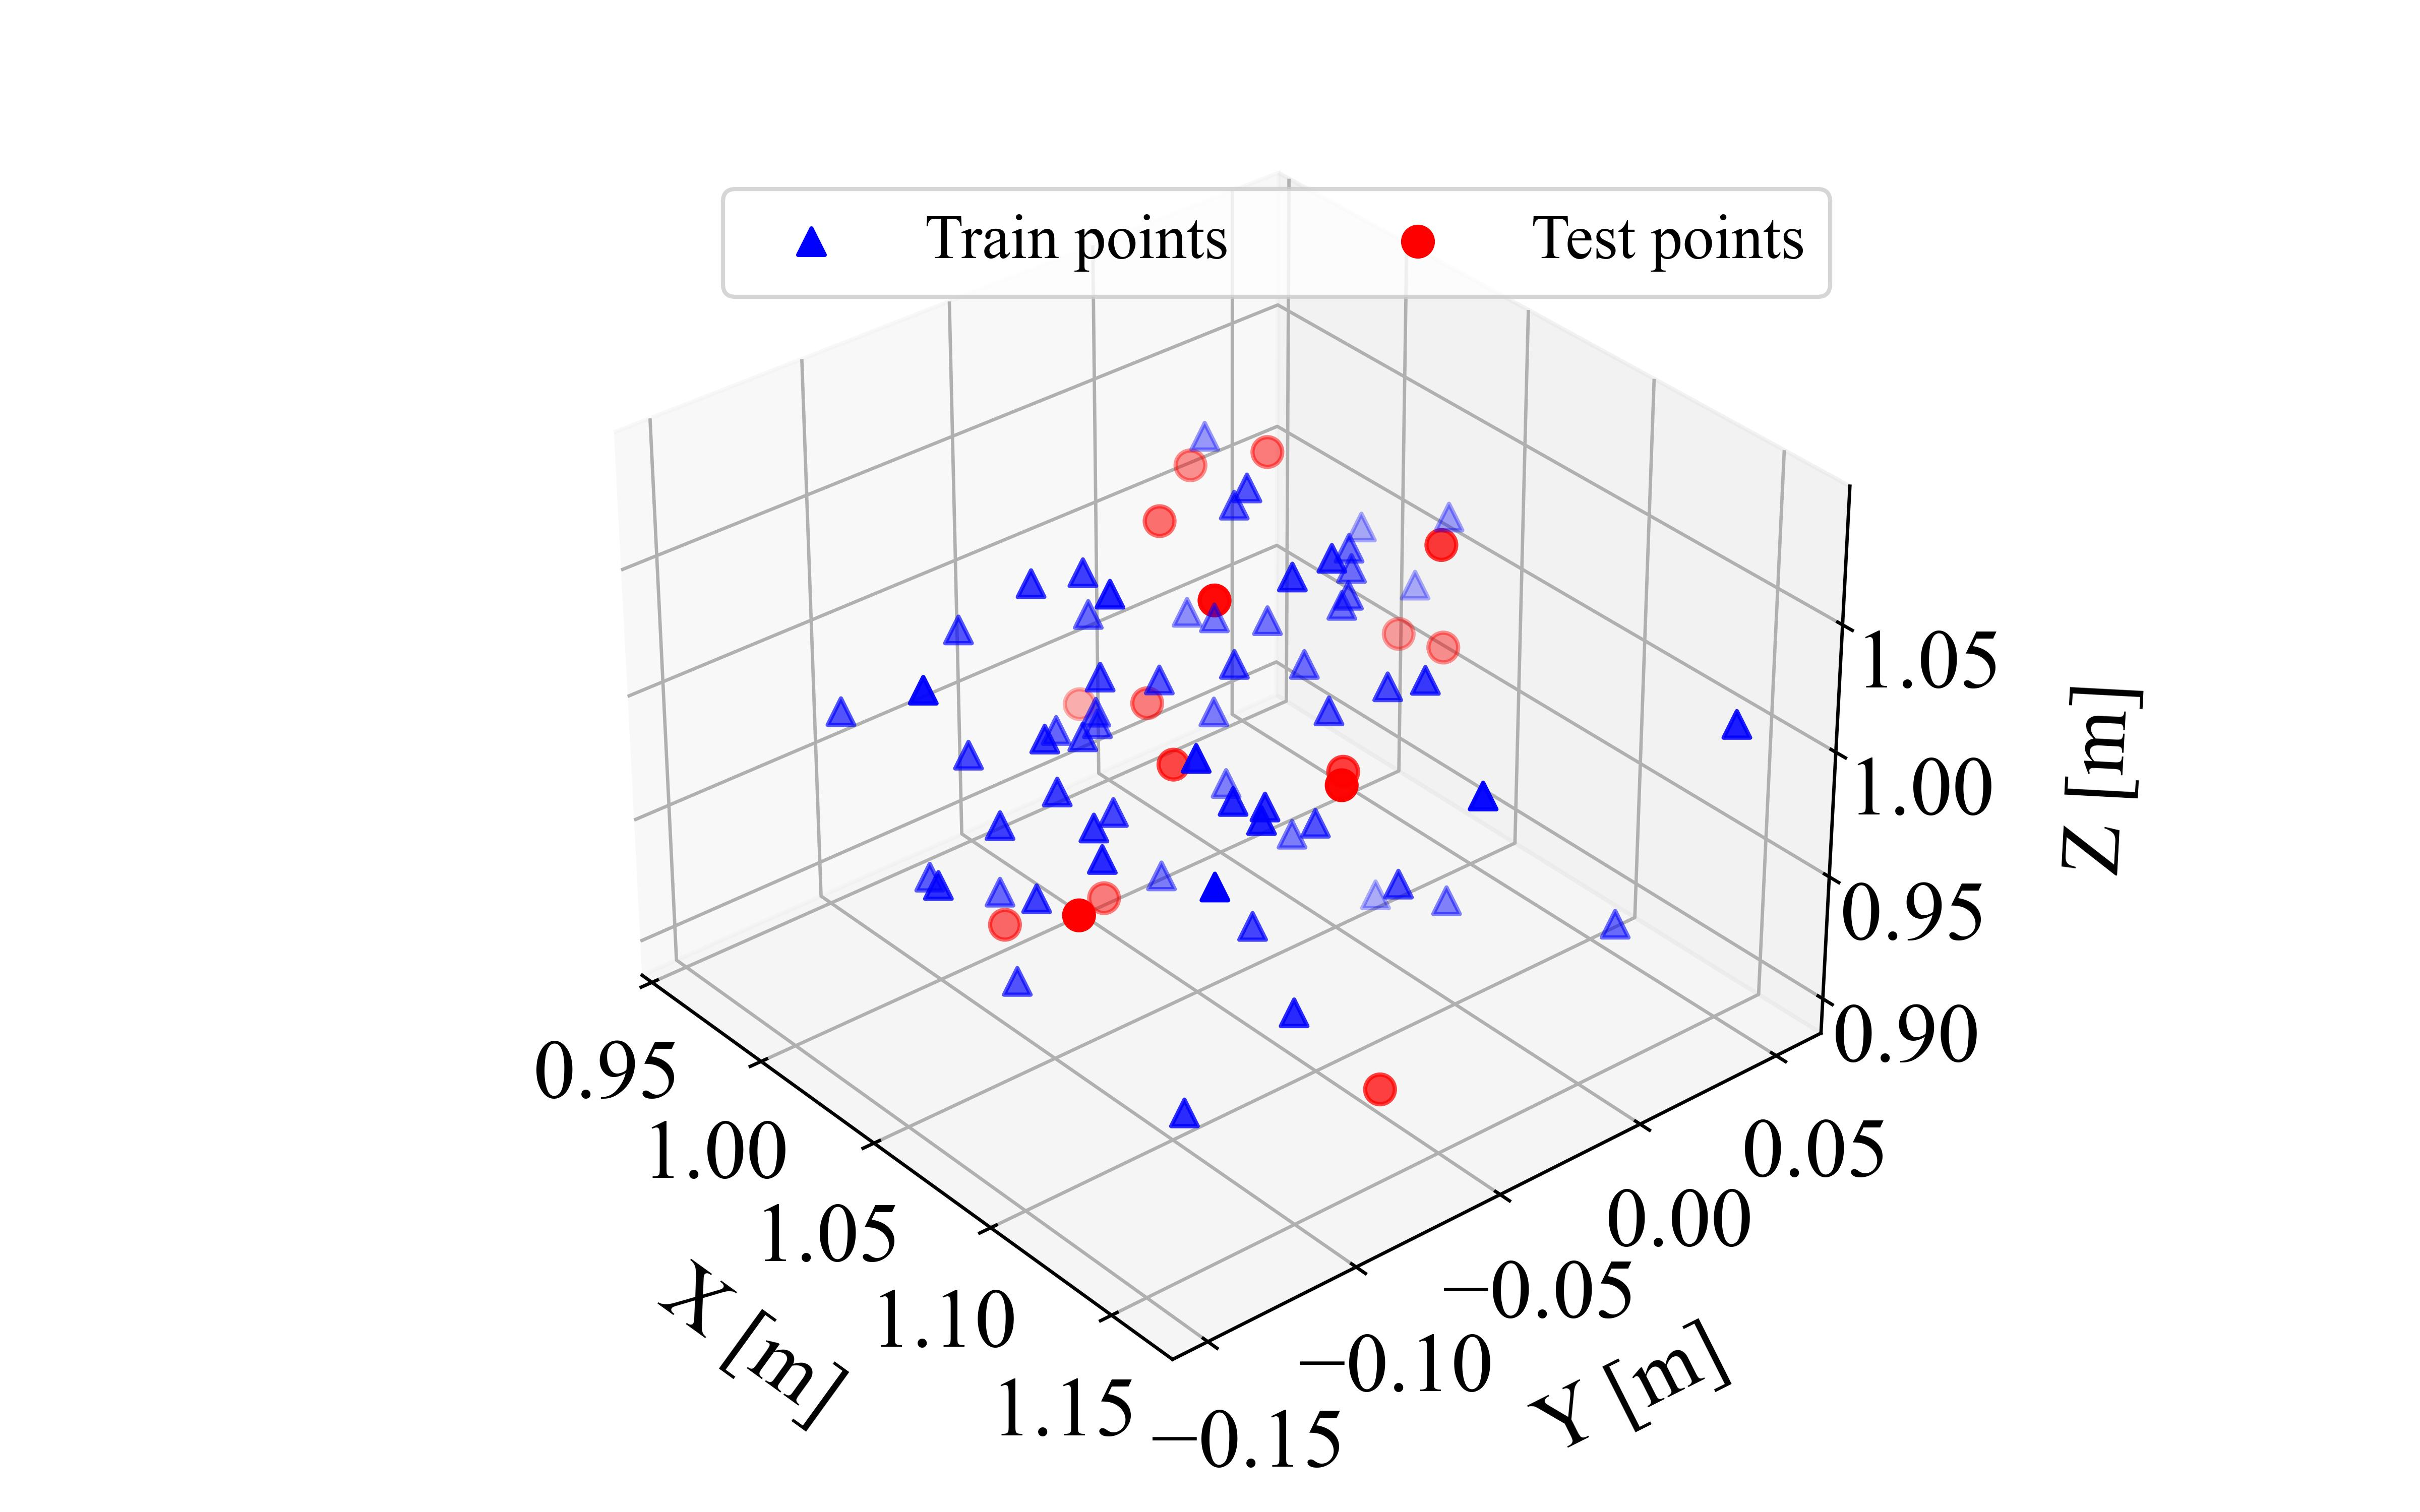
\includegraphics[width=\linewidth]{pose_distribution.jpg}
    \caption{3D spatial position distribution of the target points $\mathbf{v}_i^T$ used for synthesizing robot motion trajectories. Note: Blue triangles represent target positions in the training set, while red circles correspond to those in the test set.}
    \label{pose_dis}
\end{figure}


To comprehensively evaluate our proposed STFlowH2R model, we compare it against a range of baselines. These were selected to demonstrate a clear performance progression across different model architectures and increasingly rich visual input modalities, from 2D images to 3D point clouds.

\begin{itemize}
    \item \textbf{Implicit Behavioral Cloning (IBC)}~\cite{florence2022implicit}: A strong non-generative baseline that learns an energy function over the state-action space. The base model is evaluated using a history of RGB images and the robot's proprioceptive state. We also assess two augmented versions: \textbf{IBC+Depth}, which uses RGB-D images (a 2.5D representation), and \textbf{IBC+3D}, which operates on sequences of 3D point clouds.

    \item \textbf{BCRNN}~\cite{mandlekar2022matters}: A standard recurrent model that regresses robot actions from a sequence of observations. Similar to IBC, we evaluate it across three input modalities: the base version uses a history of RGB images and robot proprioception, \textbf{BCRNN+Depth} uses RGB-D images, and \textbf{BCRNN+3D} takes 3D point cloud sequences as input.

    \item \textbf{DP}~\cite{chi2023diffusion}: The original DP framework, adapted to take a history of RGB images of the interaction area as input. This baseline evaluates performance using standard 2D visual information. A key variant, \textbf{DP+Depth}, uses RGB-D images as input to leverage what is often termed a 2.5D representation.

    \item \textbf{DP3}~\cite{Ze2024DP3}: A state-of-the-art method that conditions a DM directly on a sequence of raw 3D point clouds, requiring the policy to learn motion dynamics implicitly from the geometric data.
\end{itemize}


\subsection{Evaluation metrics} \label{metrics}


To quantitatively assess the policies, we designed four key metrics focused on task success, efficiency, motion quality, and computational cost. Each trial terminates either when a 15-second time limit is reached or when the policy’s action plan converges, defined as the mean difference between consecutive action plans falling below 0.5 mm. Upon termination, the trial's outcome is evaluated based on the following:
\begin{itemize}
\item \textbf{Success Rate (SR):} This is the primary metric for task accomplishment. A trial is deemed successful if the final Euclidean distance between the robot's end-effector and the object's center is less than 5 cm. This practical threshold accounts for minor inaccuracies in perception and control, and we empirically verified that any final pose within this 5 cm radius allows the gripper to securely grasp and lift the object.


\item \textbf{Handover Time (HT):} This metric measures the time elapsed (in seconds) from the initiation of the robot's motion to the moment the success condition is met. It quantifies the policy's efficiency.
\item \textbf{Jerk:} This metric quantifies the smoothness of the robot's motion. It is calculated as the time-averaged integral of the squared third derivative of the end-effector's position. Lower values indicate a smoother trajectory, which is desirable for HRC.
\item \textbf{Inference Time (IT):} This metric measures the average inference time required for a single forward pass of the policy, from receiving an observation to generating an action. This quantifies the computational cost and suitability for real-time control.
\end{itemize}



\subsection{Results and analysis}   \label{results}

\subsubsection{Quantitative comparison}

In this section, we present the main quantitative results, comparing our proposed STFlowH2R model against all selected baselines. To ensure a fair and direct comparison, all methods were trained on our full, augmented dataset $\mathcal{D}_A$ and evaluated on the 24 held-out test demonstrations. The performance of all methods across the four key metrics is summarized in Table~\ref{quantitative_comparison}. The results clearly demonstrate the superiority of our STFlowH2R model. It achieves the highest SR, significantly outperforming the next best method, DP3. This indicates a substantial improvement in overall task reliability.


In terms of efficiency and motion quality, STFlowH2R also excels. It achieves the second-fastest handover time, close to the best result from DP+Depth, and is tied for the lowest Jerk with DP3, indicating that it completes the task efficiently while generating exceptionally smooth trajectories, which are inherently more predictable and thus more comfortable for a human partner. The performance gap between STFlowH2R and the strong DP3 baseline is particularly noteworthy. While both leverage 3D data, STFlowH2R's ability to explicitly model both geometric and kinematic flows provides a more structured signal for the policy compared to DP3, which must learn these dynamics implicitly from raw point clouds. The extremely low success rates of the IBC and BCRNN variants confirm that simpler non-generative or recurrent approaches struggle to handle the high-dimensional and multi-modal nature of this interaction task. As expected, baselines relying on 2D/2.5D representations like DP and DP+Depth also lag in performance, highlighting a clear trend where richer, more structured spatiotemporal representations lead to better performance on this complex interaction task.


Finally, a key consideration is the trade-off between performance and computational cost. As shown by the IT metric, our STFlowH2R model, due to its more comprehensive dual-flow encoders, is computationally more intensive than the baselines. However, its IT of approximately 48 ms (around 21 Hz) is well within the requirements for real-time control in typical handover tasks. This demonstrates that the substantial performance gains in success, efficiency, and smoothness are achieved at an acceptable computational cost.


\begin{table}[htbp]
\footnotesize
\centering
\caption{Quantitative comparison of H2R handover performance. All models are trained on $\mathcal{D}_A$. Results are reported as mean ± std over 3 seeds.}
\label{quantitative_comparison}
\begin{threeparttable}
\begin{tabular}{lcccc}
\toprule
\textbf{Method} & \textbf{SR (\%)} $\uparrow$ & \textbf{HT (s)} $\downarrow$ & \textbf{Jerk} $\downarrow$ & \textbf{IT (ms)} $\downarrow$ \\ 
\midrule
IBC                 & 5.6 ± 2.4 & 14.9 ± 0.3 & 6.3 ± 0.4 & 3.5 ± 1.1 \\
IBC+Depth           & 6.9 ± 2.4 & 14.8 ± 0.9 & 5.8 ± 1.0 & 3.6 ± 1.1 \\
IBC+3D              & 9.7 ± 4.8 & 15.0 ± 0.8 & 5.5 ± 0.6 & \textbf{2.5 ± 1.1} \\
\midrule
BCRNN               & 8.3 ± 0.0 & 14.8 ± 0.7 & 6.6 ± 0.4 & 3.9 ± 1.2 \\
BCRNN+Depth         & 12.5 ± 4.2 & 14.3 ± 0.5 & 6.4 ± 0.5 & 4.1 ± 1.1 \\
BCRNN+3D            & 15.3 ± 2.4 & 14.6 ± 1.8 & 5.1 ± 0.8 & 3.2 ± 1.0 \\
\midrule
DP                  & 26.4 ± 2.4 & 13.1 ± 1.5 & 4.6 ± 0.8 & 46.4 ± 11.5 \\
DP+Depth            & 48.6 ± 2.4 & \textbf{10.1 ± 2.1} & 4.7 ± 0.9 & 47.4 ± 10.9 \\
DP3                 & 69.4 ± 4.8 & 11.1 ± 1.8 & \textbf{4.5 ± 0.7} & 46.4 ± 15.6 \\    
\midrule
\textbf{STFlowH2R}  & \textbf{87.5 ± 4.2} & 10.3 ± 2.1 & \textbf{4.5 ± 0.7} & 47.9 ± 5.4 \\
\bottomrule
\end{tabular}
\begin{tablenotes}
\footnotesize
\item[1] \textbf{Bold} indicates the best performance.
\end{tablenotes}
\end{threeparttable}
\end{table}


\subsubsection{Ablation study}
To systematically investigate the key sources of its performance, we conduct a series of ablation studies. We investigate two primary aspects: (1) the impact of our proposed data generation and augmentation pipeline, and (2) the contribution of the core architectural components within our STFlowH2R model.


\paragraph{Impact of Data Generation and Augmentation}
First, we evaluate the effectiveness of our data generation strategy. We trained our STFlowH2R model and the strongest baseline, DP3, on the three different datasets: the basic dataset $\mathcal{D}_B$, the multi-trajectory dataset $\mathcal{D}_M$, and our full augmented dataset $\mathcal{D}_A$. The results in Table~\ref{data_ablation} show a consistent improvement across all metrics as the training data becomes richer. This comprehensive improvement shows that our data augmentation strategy helps the models find more successful solutions and also teaches them to generate policies that are fundamentally more efficient and smoother. This confirms that exposing the models to diverse spatial and temporal interaction patterns is key to learning high-quality, reliable handover behaviors.


\begin{table}[htbp]
\footnotesize
\centering
\caption{Performance impact of data augmentation strategies. Results are reported as mean ± std over 3 seeds.}
\label{data_ablation}
\begin{threeparttable}
\begin{tabular}{llccc}
\toprule
\textbf{Model} & \textbf{Dataset} & \textbf{SR (\%)} $\uparrow$ & \textbf{HT (s)} $\downarrow$ & \textbf{Jerk} $\downarrow$ \\
\midrule
\multirow{3}{*}{DP3} 
& $\mathcal{D}_B$ & 43.1 ± 6.4 & 11.9 ± 2.0 & 5.0 ± 0.9 \\
& $\mathcal{D}_M$ & 50.0 ± 4.2 & 11.7 ± 1.9 & 4.8 ± 0.7 \\
& $\mathcal{D}_A$ & 69.4 ± 4.8 & 11.1 ± 1.8 & 4.5 ± 0.6 \\
\midrule
\multirow{3}{*}{\textbf{STFlowH2R}} 
& $\mathcal{D}_B$ & 63.9 ± 2.4 & 10.9 ± 2.1 & 4.9 ± 0.7 \\
& $\mathcal{D}_M$ & 76.4 ± 6.4 & 10.7 ± 2.1 & 4.8 ± 0.7 \\
& $\mathcal{D}_A$ & \textbf{87.5 ± 4.2} & \textbf{10.3 ± 2.1} & \textbf{4.5 ± 0.7} \\
\bottomrule
\end{tabular}
\begin{tablenotes}
\item[*] The datasets are progressively enriched, starting with $\mathcal{D}_B$ (basic, one trajectory per demonstration), then $\mathcal{D}_M$ (adding spatial augmentation via multiple trajectories), and finally $\mathcal{D}_A$ (adding temporal augmentation).
\end{tablenotes}
\end{threeparttable}
\end{table}

\paragraph{Architectural Ablation of STFlowH2R}
Next, we analyze the architectural choices within our STFlowH2R model. We created three ablated versions of the model and trained them on the full dataset $\mathcal{D}_A$ to isolate the contribution of each key component.

\begin{itemize}
    \item \textbf{w/o Skeletal Flow}: This version removes the skeletal kinematic flow encoder $\mathcal{F}_S$, forcing the policy to rely solely on our ICP-aligned geometric flow for its understanding of the scene's dynamics.

    \item \textbf{w/o ICP Alignment}: In this variant, we feed the raw, unaligned point cloud sequence directly to the geometric encoder, bypassing the ICP registration step. This allows us to isolate the specific benefit of explicitly modeling geometric motion through temporal alignment.

    \item \textbf{w/o Geometric Flow}: This version removes our proposed geometric motion flow encoder $\mathcal{F}_G$. Instead of the structured geometric flow, the policy is conditioned on the skeletal flow and raw RGB-D images processed by a visual encoder. This baseline tests the value of our explicit geometric motion representation against a more conventional vision-based input.
\end{itemize}

\begin{table}[htbp]
\footnotesize
\centering
\caption{Architectural ablation of the STFlowH2R model. All variants are trained on $\mathcal{D}_A$. Results are reported as mean ± std over 3 seeds.}
\label{arch_ablation}
\begin{tabular}{lcccc}
\toprule
\textbf{Variant} & \textbf{SR (\%)} $\uparrow$ & \textbf{HT (s)} $\downarrow$ & \textbf{Jerk} $\downarrow$ & \textbf{IT (ms)} $\downarrow$ \\ 
\midrule
\textbf{STFlowH2R (Full)} & \textbf{87.5 ± 4.1} & \textbf{10.3 ± 2.1} & \textbf{4.5 ± 0.7} & 47.9 ± 5.4 \\
w/o Skeletal Flow         & 75.0 ± 4.1 & 10.5 ± 2.0 & 4.6 ± 0.8 & \textbf{45.8 ± 3.2} \\
w/o ICP Alignment         & 68.0 ± 2.4 & 10.5 ± 2.1 & 4.6 ± 0.7 & 47.8 ± 4.9 \\
w/o Geometric Flow        & 56.9 ± 2.4 & 10.6 ± 2.2 & 4.9 ± 1.0 & 48.9 ± 8.4 \\
\bottomrule
\end{tabular}
\end{table}

The results in Table~\ref{arch_ablation} validate our architectural design and clarify the distinct contribution of each component to the model's overall performance. As expected, removing the geometric flow leads to a severe performance collapse, confirming that our explicit geometric motion representation is the most essential component for reliable task completion. The impact of the other two components is also significant, primarily impacting the task success rate; removing either the skeletal flow or the explicit ICP alignment results in a substantial drop in SR. The crucial contribution of the geometric flow becomes evident not only in reliability but also in motion quality, as its removal leads to the most substantial increase in Jerk. This demonstrates how each component plays a distinct role: (1) the geometric motion flow is indispensable for both high success rates and smooth motion; (2) the skeletal kinematic flow provides high-level contextual cues about human motion that are critical for robust policy learning; and (3) the ICP alignment is similarly vital for understanding object dynamics to ensure successful completion. Notably, these significant performance differences do not come at a computational trade-off, as the inference times across all variants are highly comparable. This confirms that the superior performance of the full STFlowH2R model is a direct result of its comprehensive, multi-flow architecture, which strikes the best overall balance by synergistically integrating all components.


\subsubsection{Sensitive analyses}

To investigate the robustness of our STFlowH2R model and provide empirical support for our choice of key hyperparameters, we conduct a sensitivity analysis on the observation horizon $T_o$ and the action execution horizon $T_a$. For this specific analysis, we set the prediction horizon to $T_p=16$ to allow for a wider range of parameter sweeps. All experiments are performed with the full model trained on the augmented dataset $\mathcal{D}_A$, and results are reported as the mean and standard deviation over 3 random seeds. The results are visualized in Fig.~\ref{sensitivity_analysis}.

\begin{figure}[htbp]
    \centering
    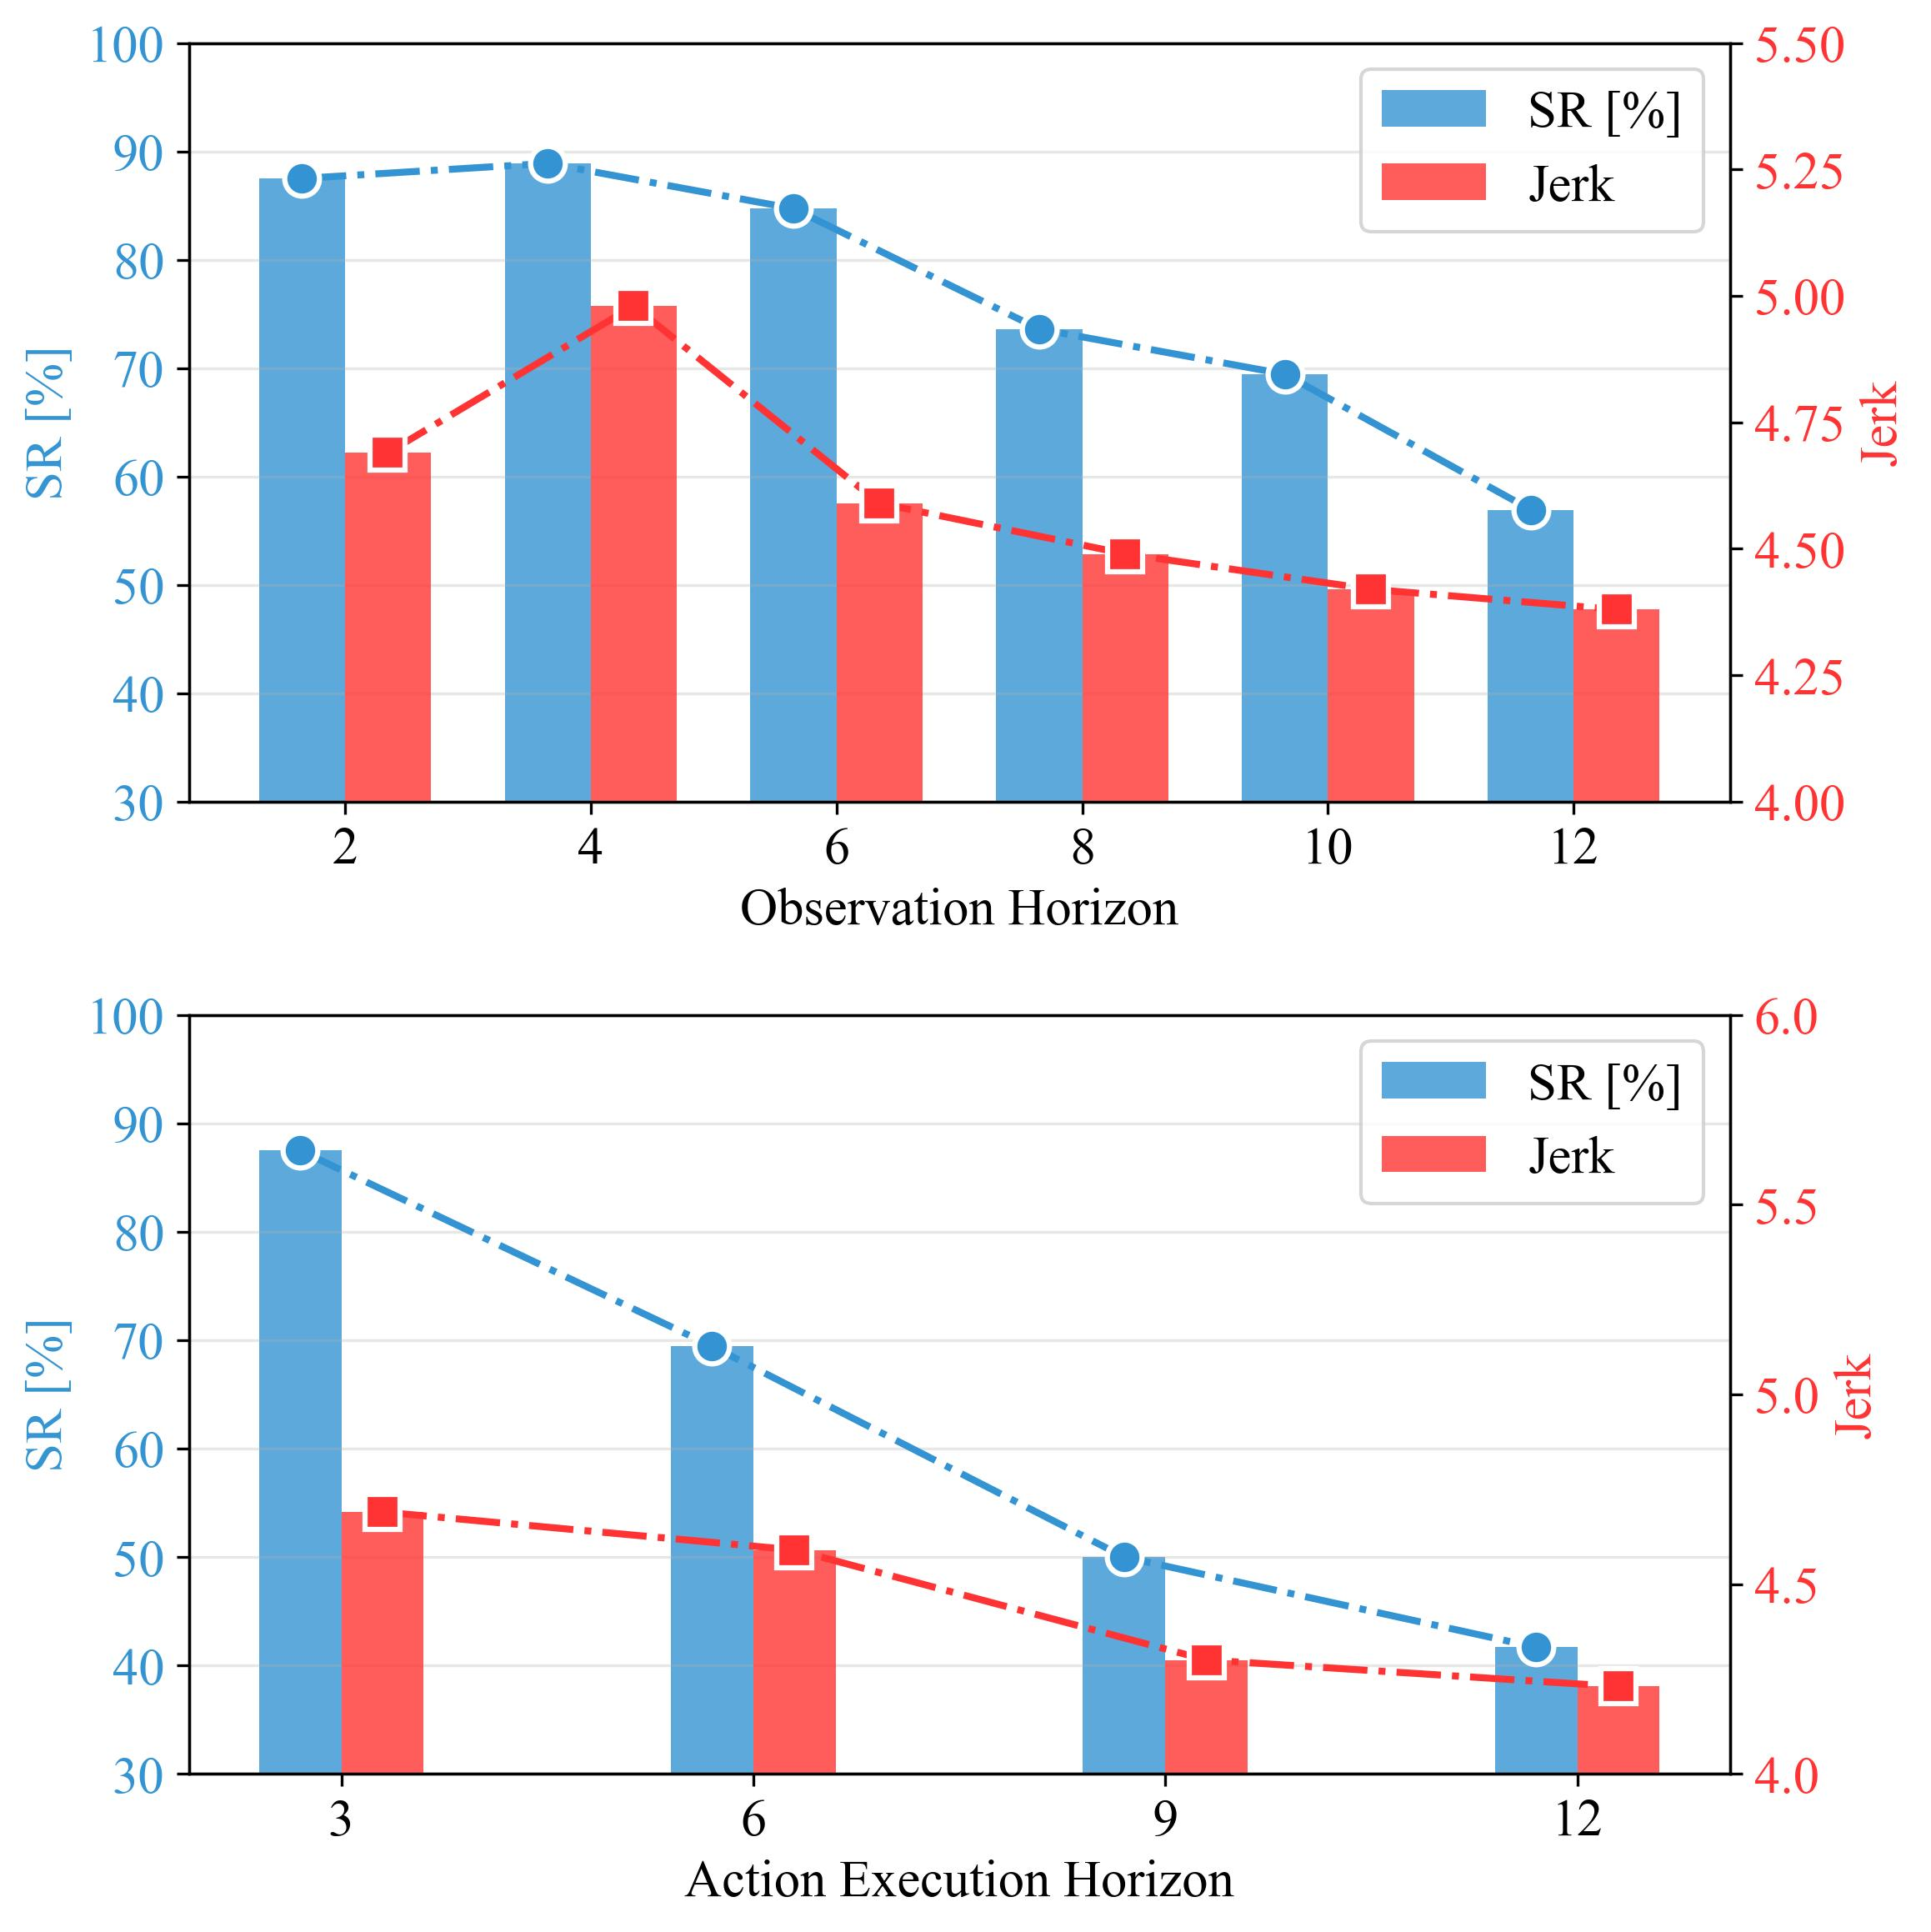
\includegraphics[width=\linewidth]{sensitivity_analysis.jpg}
    \caption{Sensitivity analysis of key hyperparameters, showing the trade-off between SR and Jerk. (a) Impact of the observation horizon ($T_o$) on performance, with $T_p=16$ and $T_a=3$ fixed. (b) Impact of the action execution horizon ($T_a$) on performance, with $T_p=16$ and $T_o=2$ fixed.}
    \label{sensitivity_analysis}
\end{figure}


\paragraph{Sensitivity to Observation Horizon $T_o$}
The observation horizon $T_o$ determines how much past information the policy uses to make a decision. A sufficient history is crucial for understanding human intent, but an overly long horizon may introduce irrelevant information. We varied $T_o$ from 2 to 12, while keeping the prediction horizon fixed at $T_p=16$ and the action execution horizon at $T_a=3$. As shown in Fig.~\ref{sensitivity_analysis}(a), the success rate exhibits an inverted U-shape. The model achieves a high success rate even with $T_o=2$, peaks with a marginal improvement at $T_o=4$, and then performance steadily degrades as the horizon becomes excessively long. This suggests that a brief context is sufficient for near-optimal performance, whereas overly long histories introduce irrelevant noise. The Jerk follows a more complex trend, with an unexpected spike at $T_o=4$, which coincides with the peak success rate. This suggests a potential trade-off: the optimal observation horizon for task success may encourage a more aggressive and decisive policy, which, while effective, results in less smooth motion. As the observation horizon lengthens further, the policy becomes more conservative, and the Jerk subsides, reaching its minimum at $T_o=12$. This analysis strongly validates our choice of $T_o=2$ for the main experiments. Although $T_o=4$ achieves the peak success rate, the performance gain compared to $T_o=2$ is marginal. This minor improvement in success comes at the cost of a substantial degradation in motion quality, as the Jerk at $T_o=4$ is significantly higher. Therefore, $T_o=2$ strikes a superior balance between high reliability and smooth, natural motion.



\paragraph{Sensitivity to Action Execution Horizon $T_a$}
The action execution horizon $T_a$, within a receding horizon control framework, governs the trade-off between policy reactivity and motion smoothness. The prediction horizon was fixed at $T_p=16$ and the observation horizon at $T_o=2$, while $T_a$ was varied from 3 to 12. The results, shown in Fig.~\ref{sensitivity_analysis}(b), demonstrate a classical trade-off. The success rate peaks at the shortest execution horizon $T_a=3$ and decreases monotonically as $T_a$ increases. This underscores the critical role of reactivity in the dynamic H2R handover task. A shorter $T_a$ enables more frequent re-planning, allowing the robot to continuously adapt to subtle variations in the human partner’s motion and thereby maximize task success. In contrast, motion smoothness exhibits the opposite trend. Jerk decreases monotonically with increasing $T_a$, yielding the smoothest trajectory at the longest execution horizon $T_a=12$. This confirms that executing longer, uninterrupted plans generated by the DM produces more coherent and fluid motions, while frequent re-planning introduces minor jerkiness due to the stitching of action segments. This analysis empirically supports the choice of $T_a=3$ and $T_p=4$ for the main experiments. Since task completion is the primary objective, the significant gain in success rate achieved by a highly reactive policy justifies the modest compromise in motion smoothness.


\subsubsection{Qualitative analysis}
To provide a more intuitive understanding of the model's performance, we first examine the trajectories generated by the STFlowH2R policy in a simulation environment and subsequently illustrate the successful real-world execution of these learned behaviors.


Fig.~\ref{fig:sim_results} presents a representative end-effector trajectory from simulation, comparing the resulting motion from the policy's direct actions against that from a temporally smoothed action. The direct trajectory is generated by executing the raw action sequence from the STFlowH2R policy. The position curves are continuous with gentle slopes, confirming the policy’s ability to produce low-jerk motion profiles as reported in our quantitative analysis. Notably, the Z-axis exhibits a distinct arc-like shape, indicating that the policy has acquired a top-down handover strategy tailored for HRC, which proactively reduces the risk of collision with the human partner’s arm. The smoothed trajectory is generated by first applying a temporal averaging filter to the policy's raw output action sequence and then executing the resulting smoothed action. As the comparison illustrates, this post-processing of the actions effectively removes minor high-frequency oscillations—inherent in the re-planning process—from the final end-effector trajectory, yielding a visibly smoother path. This analysis demonstrates that while the base policy generates robust and intelligent action plans, the resulting motion quality can be further enhanced when exceptional smoothness is required.


\begin{figure}[!htb]
    \centering
    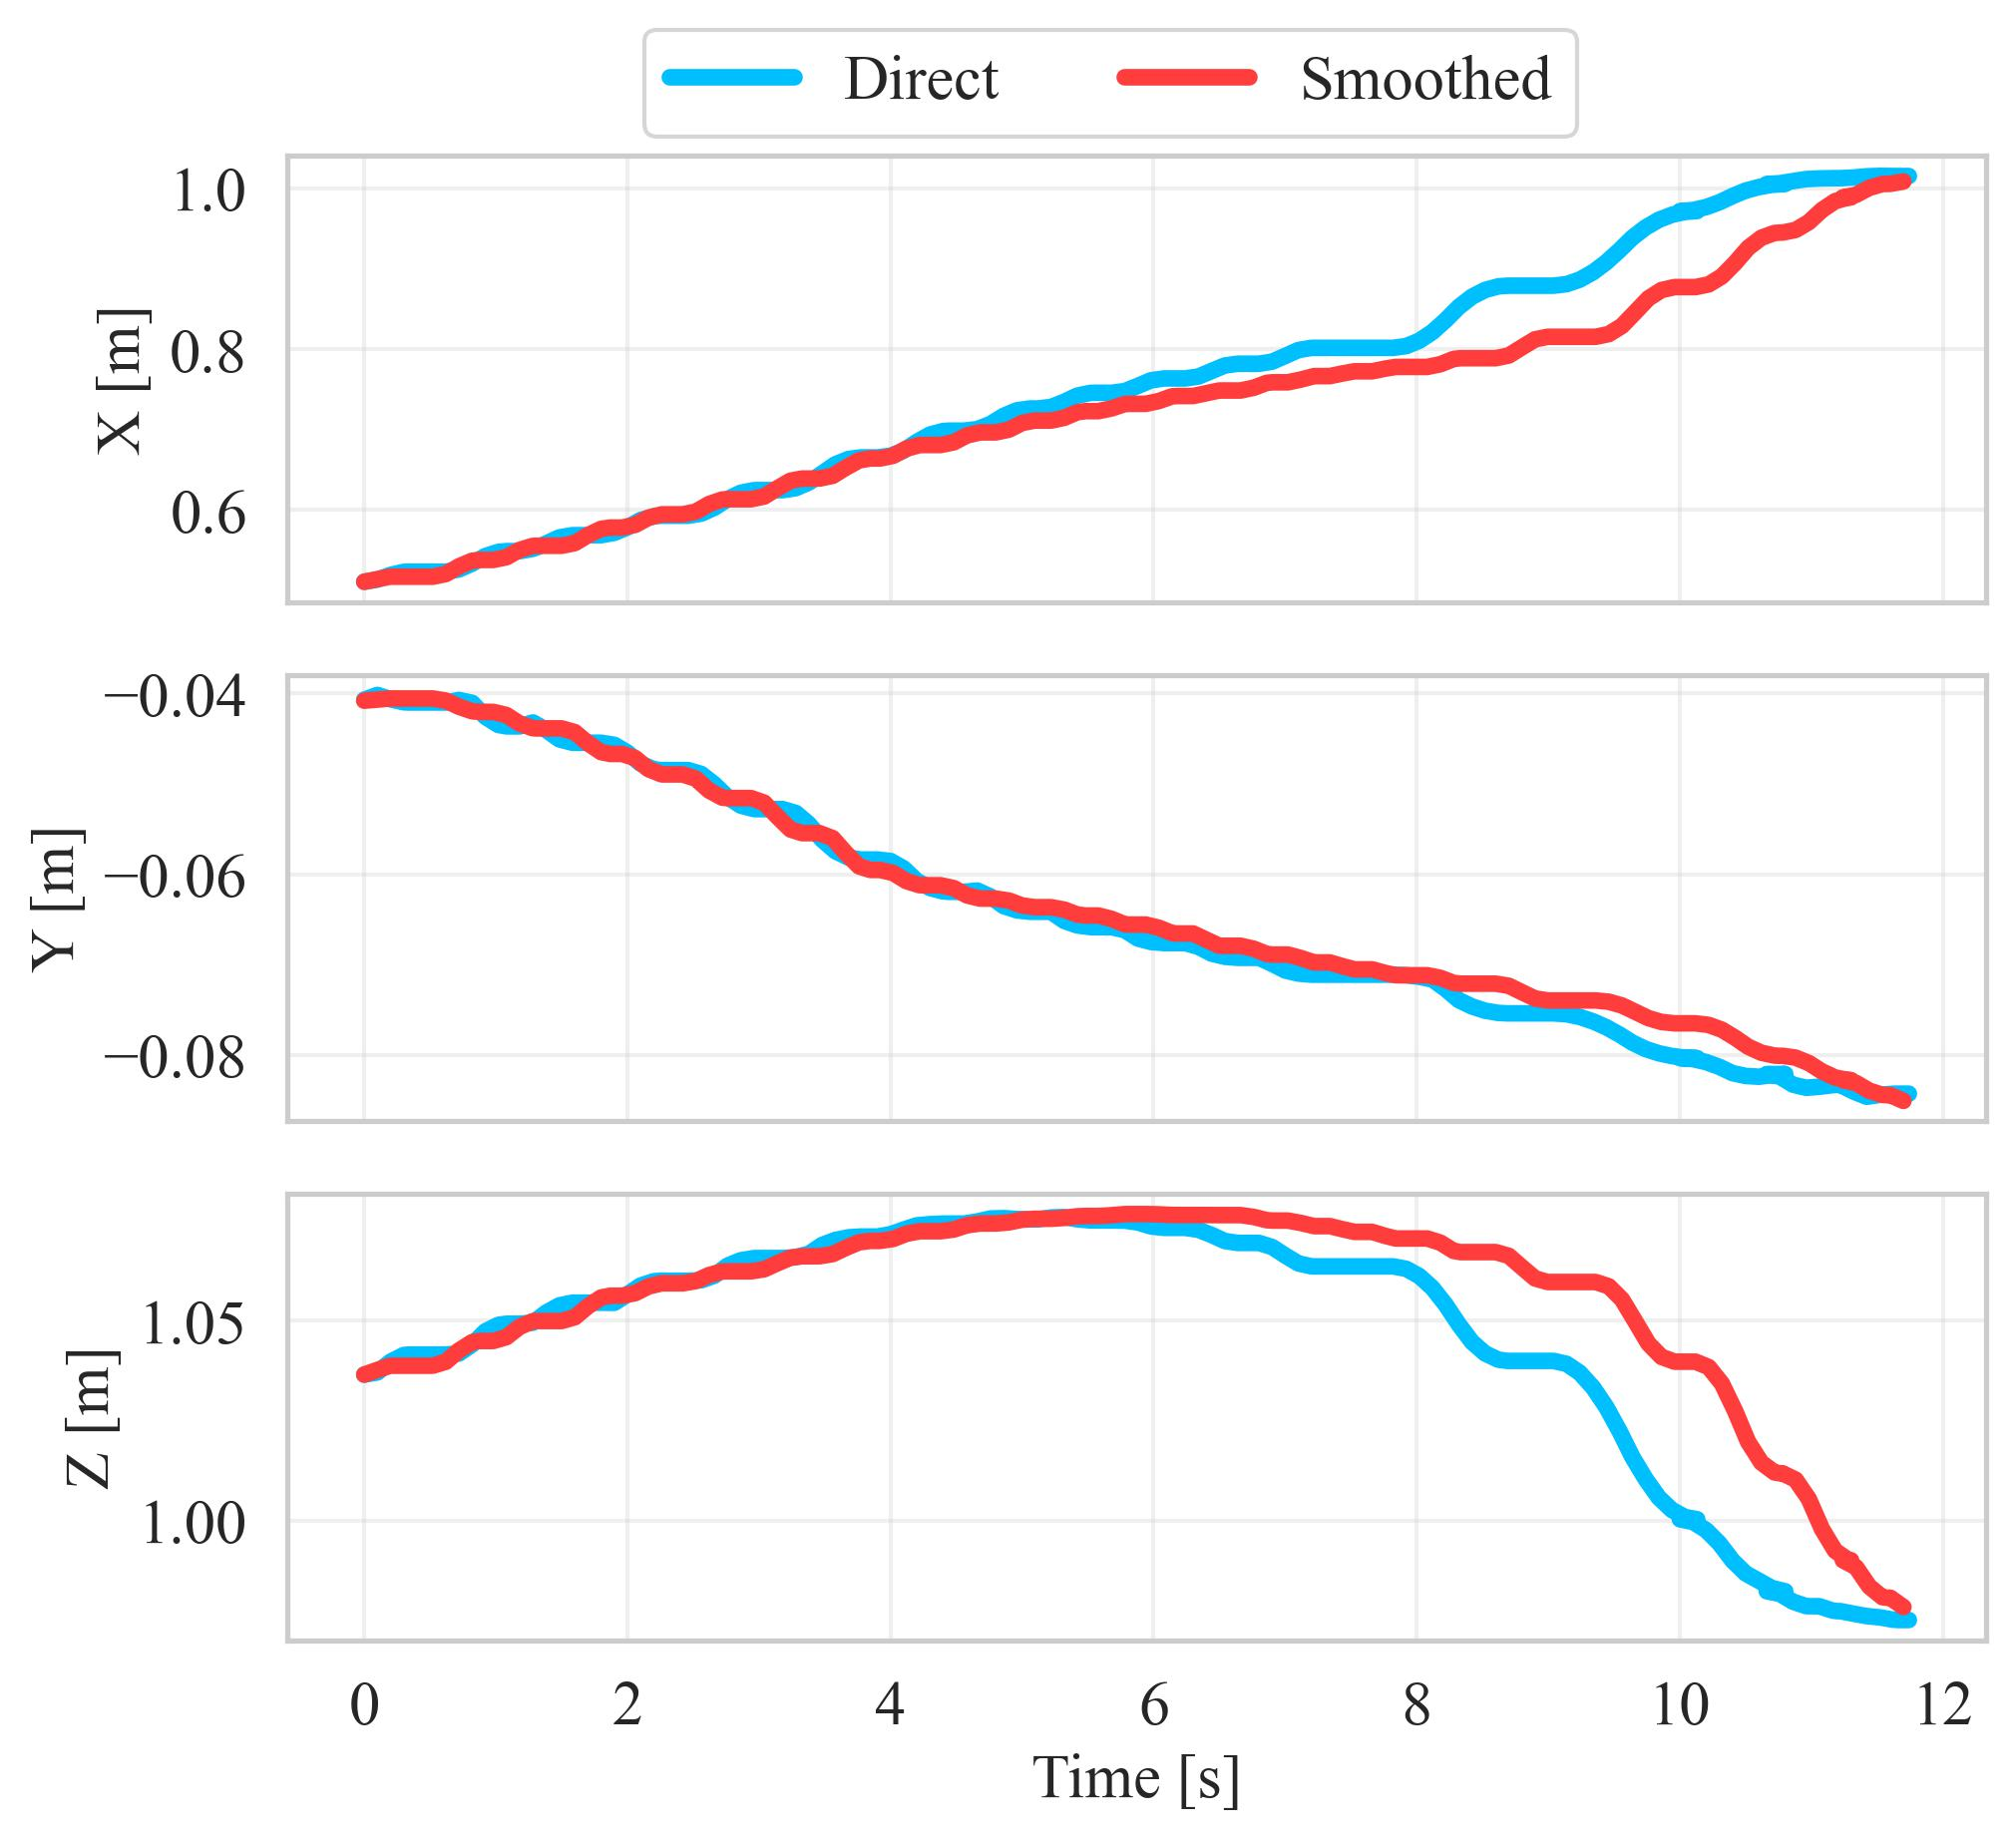
\includegraphics[width=0.8\linewidth]{sim_results.jpg}
    \caption{Comparison of end-effector trajectories generated by the STFlowH2R policy. The blue curve represents the trajectory obtained by directly executing the raw policy output, while the red one corresponds to the trajectory after applying temporal smoothing to the actions.}
    \label{fig:sim_results}
\end{figure}

Subsequently, we demonstrate the successful execution of these behaviors in a real-world H2R handover task, as illustrated in Fig.~\ref{fig:qualitative_analysis}. The complete task sequence comprises the policy-driven reaching motion, gripper activation, and a predefined movement toward the drop-off location. The panoramic snapshots (a) and the robot’s perception view (b) reveal a smooth and anticipatory motion. From the initial state, the robot arm proactively initiates a trajectory toward the anticipated handover location, synchronizing seamlessly with the human partner’s movement. This successful physical deployment directly reflects the well-structured trajectories analyzed in simulation. Overall, the combined qualitative evidence confirms that the proposed STFlowH2R policy not only completes the handover task effectively but also does so in an efficient and natural manner suited to HRC scenarios.

\begin{figure*}[!htb]
    \centering
    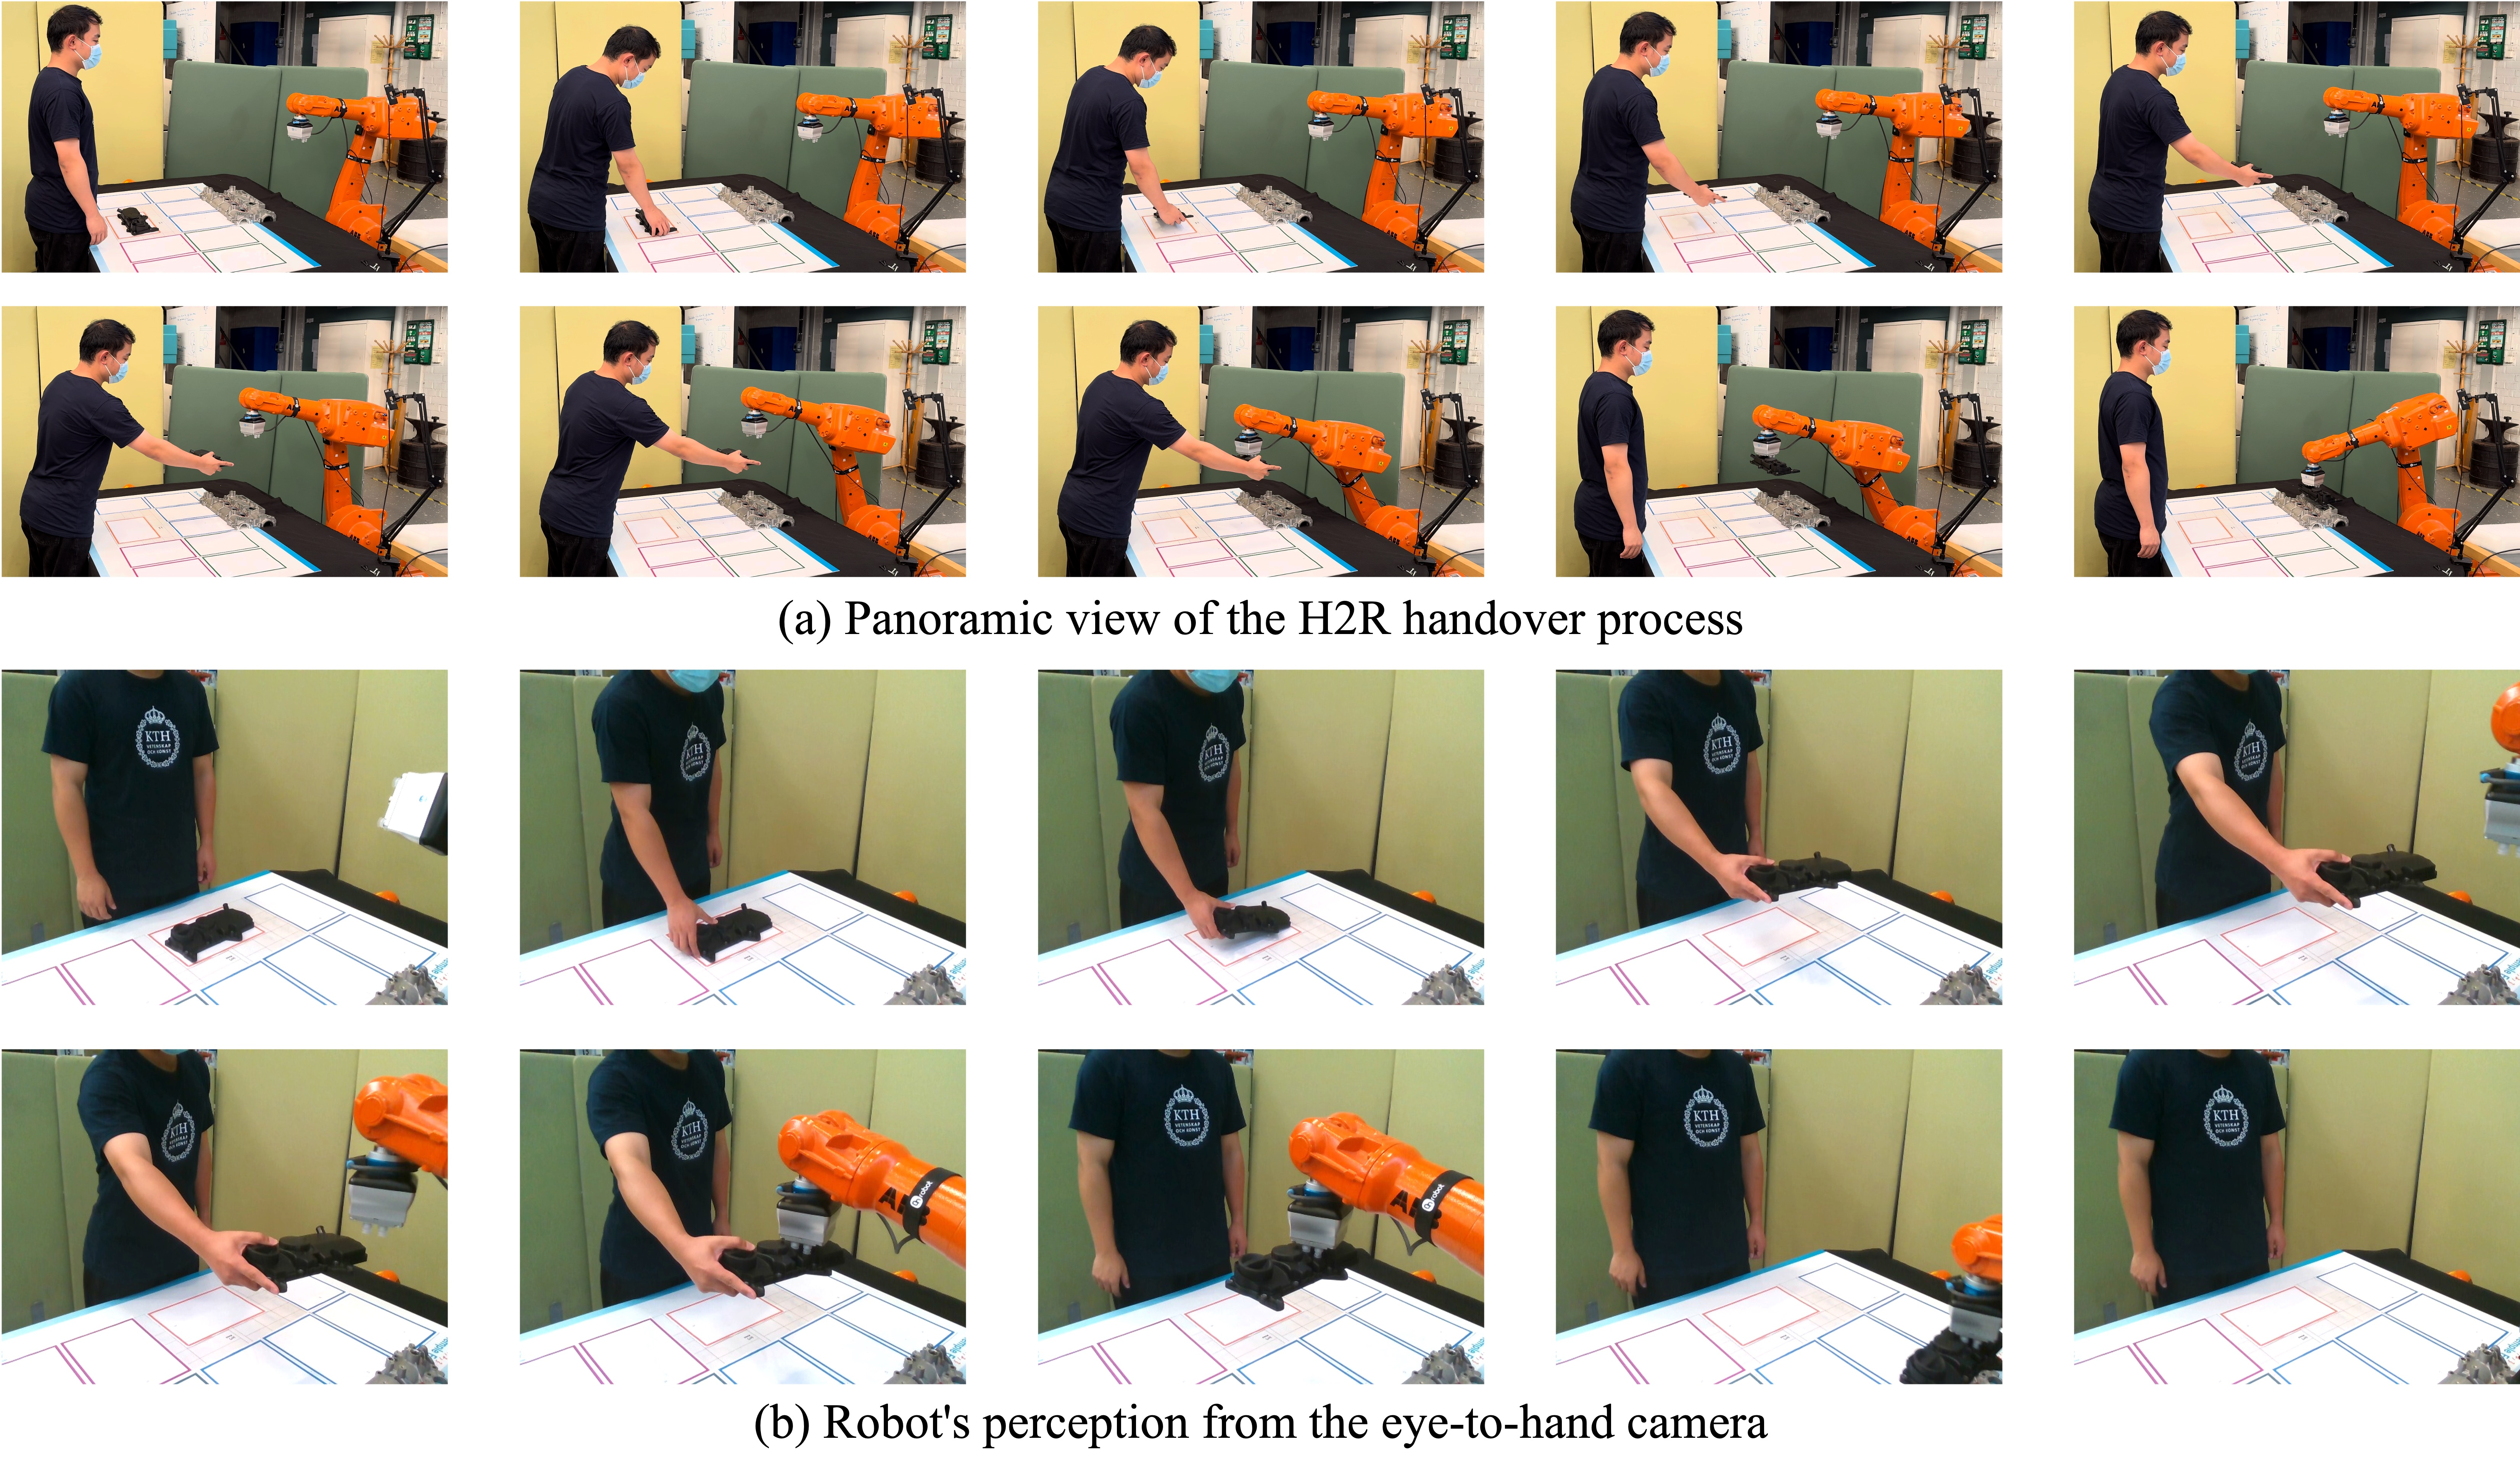
\includegraphics[width=\linewidth]{physical_results.jpg}
    \caption{Qualitative analysis of the STFlowH2R policy in a real-world H2R handover experiment. The figure illustrates a successful handover process, showing: (a) a panoramic view of the shared workspace in HRC; and (b) the corresponding robot's perception from the eye-to-hand camera}
    \label{fig:qualitative_analysis}
\end{figure*}


%% ------------------------------------------------------------------------------------------
\section{Conclusion} \label{sec:5}
In this paper, we presented a two-stage framework to address the significant challenges of data scarcity and inadequate state representation in learning robust policies for H2R object handover tasks. Our primary contribution is a novel approach that decouples data generation from physical robot interaction and leverages a rich, structured representation of the dynamic handover scene. The first stage of our framework introduces an offline, physical robot-free data generation pipeline. By combining VFMs-based pose estimation with programmatic motion synthesis and rule-based temporal alignment, this pipeline efficiently produces a large-scale, diverse dataset of handover demonstrations, effectively mitigating the high cost and labor associated with traditional data collection methods. The second stage of our framework proposes the STFlowH2R policy. This diffusion-based model is conditioned on a novel 4D spatiotemporal flow representation. We demonstrated that by explicitly modeling both high-level skeletal kinematics and fine-grained, ICP-aligned geometric motion, our policy can generate actions that are not only successful but also efficient. Our extensive experiments validate the proposed framework, showing that STFlowH2R achieves an 87.5\% task success rate—18.1 percentage points higher than the strongest baseline—and attains state-of-the-art efficiency (10.3 s handover time) and motion smoothness (4.5 Jerk). Furthermore, our ablation studies empirically confirmed that both the data augmentation strategy and the individual components of our 4D spatiotemporal flow representation are critical to the final performance.

Despite these promising results, this work has limitations that open avenues for future research. First, the current framework relies on 3D position control for the end-effector and focuses on a single object type, which limits its broader applicability. Future work should therefore focus on augmenting the action space with orientation control and generalizing the policy across a diverse set of objects with varied geometries. Second, future work should improve the policy's robustness in dynamic H2R handovers. Finally, the fidelity of our learned policy is intrinsically linked to the quality of the offline data generation pipeline. This reliance introduces potential constraints, including the accuracy of the VFMs-based object pose estimation under challenging visual conditions and the fact that our synthesized robot trajectories, while diverse and kinematically valid, may not fully capture the nuances of optimal or human-like motion. Future research could investigate methods to refine these synthetic datasets with a small amount of real-world data or explore more advanced generative models for trajectory synthesis.


\section*{CRediT authorship contribution statement}
\textbf{Ruirui Zhong:} Conceptualization, Investigation, Methodology, Writing - Original Draft, Visualization. \textbf{Bingtao Hu}: Conceptualization, Methodology, Writing - Review \& Editing, Supervision. \textbf{Zhihao Liu}: Methodology, Software, Writing - Review \& Editing. \textbf{Qiang Qin}: Data Curation, Writing - Review \& Editing. \textbf{Yixiong Feng}: Writing - Review \& Editing, Supervision. \textbf{Xi Vincent Wang}: Conceptualization, Methodology, Writing - Review \& Editing, Supervision. \textbf{Lihui Wang}:  Writing - Review \& Editing, Supervision. \textbf{Jianrong Tan}:  Writing - Review \& Editing, Supervision.

\section*{Declaration of competing interest}
The authors declare that they have no known competing financial interests or personal relationships that could have appeared to influence the work reported in this paper.

\section*{Acknowledgments}
This work was supported in part by the National Key Research and Development Program of China under Grant No. 2024YFB3311803, and the National Natural Science Foundation of China under Grant No. 52205288.


\bibliographystyle{elsarticle-num}
\bibliography{ref}

\end{document}